% -*- program : pdflatex -*-
\documentclass{article}

\usepackage[utf8x]{inputenc}
\usepackage[T1]{fontenc}

\usepackage[margin=1.15in]{geometry}

\usepackage{fancyvrb}
\usepackage{mathtools}
% \usepackage{tikz}
\usepackage{graphicx}
\usepackage{epstopdf}

% For the degree circle sign
\usepackage{textcomp}

\usepackage{lmodern}
\usepackage{hyperref}

\usepackage{placeins}
% \usepackage[numbered, framed]{../../Libraries/mcode}
\usepackage{listings}

\usepackage{float}
\usepackage[list=true]{subcaption}

\newcommand{\xt}[1]{\texttt{#1}}
\newcommand{\quotes}[1]{``#1''}
\newcommand{\TW}{\textwidth}

% \includeonly{chapters/advanced_techniques}

\begin{document}

    \title{Web GUI for \\ L-System}
    \author{Chiciuc Nicușor}
    \maketitle

    
    % \pagebreak
    \tableofcontents

    \section{Introduction}
    The following paper will discuss a special case of L-Systems using a program written by the author.


	\subsection{General Iterative Function Systems}
    L-Systems are a method for constructing fractals. 


    \section{Demonstration}

    \subsection{An colorful approach}

        Suppose we have the following transformation (Figure~\ref{simple01}).
        
        % \begin{figure}[ht]
        %     \caption{A simple transformation.}
        %     \label{simple01}
        %     \centering
        %     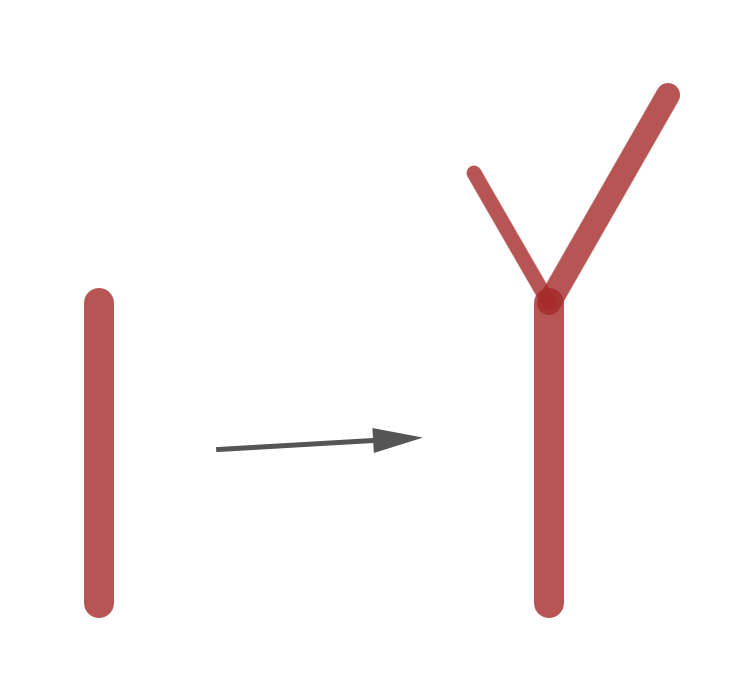
\includegraphics[width=0.15\textwidth]{img/simple01.png}
        % \end{figure}
        % \FloatBarrier

        That is, transform a segment into a branch composed of three segments.
        This process can be applied to the two smaller branches.
        Repeating this process some numbers of times reveals a beautiful, fractal pattern (Figure~\ref{simple02}).
        This pattern is very similar to the \emph{Barnsley fern} \cite{barnsley_fern}.

        \begin{figure}[ht]
            \centering
            \caption{First steps.}
            \subcaptionbox{\label{simple01} A simple transformation.}[0.45\textwidth]
                {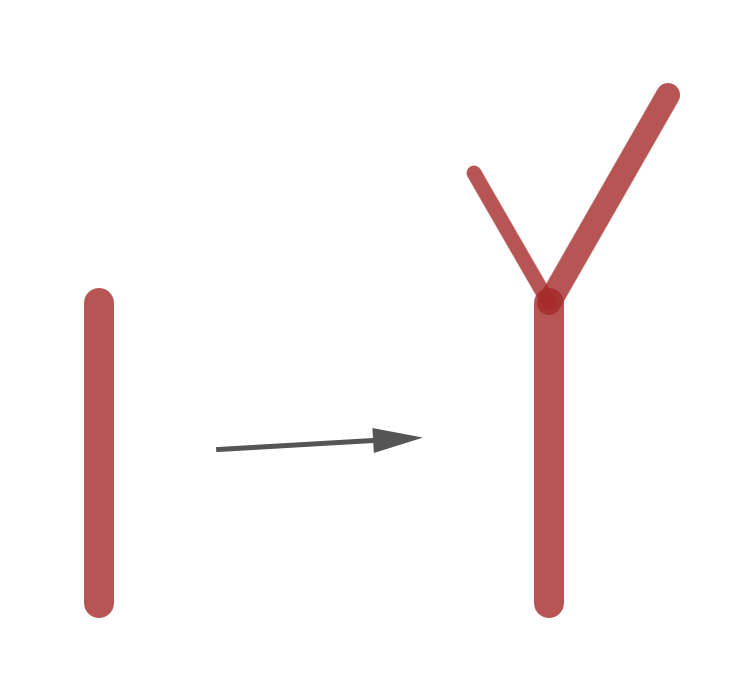
\includegraphics[width=0.2\textwidth]{img/simple01.png}}
            ~
            \subcaptionbox{\label{simple02} Several level of recursion.}[0.45\textwidth]
                {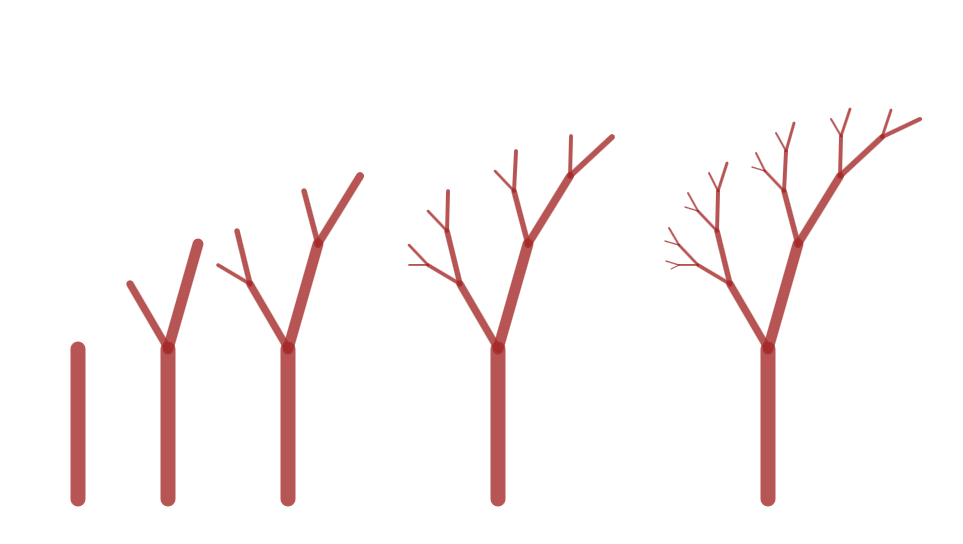
\includegraphics[width=0.4\textwidth]{img/simple02.png}}            
        \end{figure}
        \FloatBarrier

        A much more detailed rendering can be observed in Figure~\ref{simple03}

        \begin{figure}[ht]
            \caption{\label{simple03} A deeper recursion level.}
            \centering
            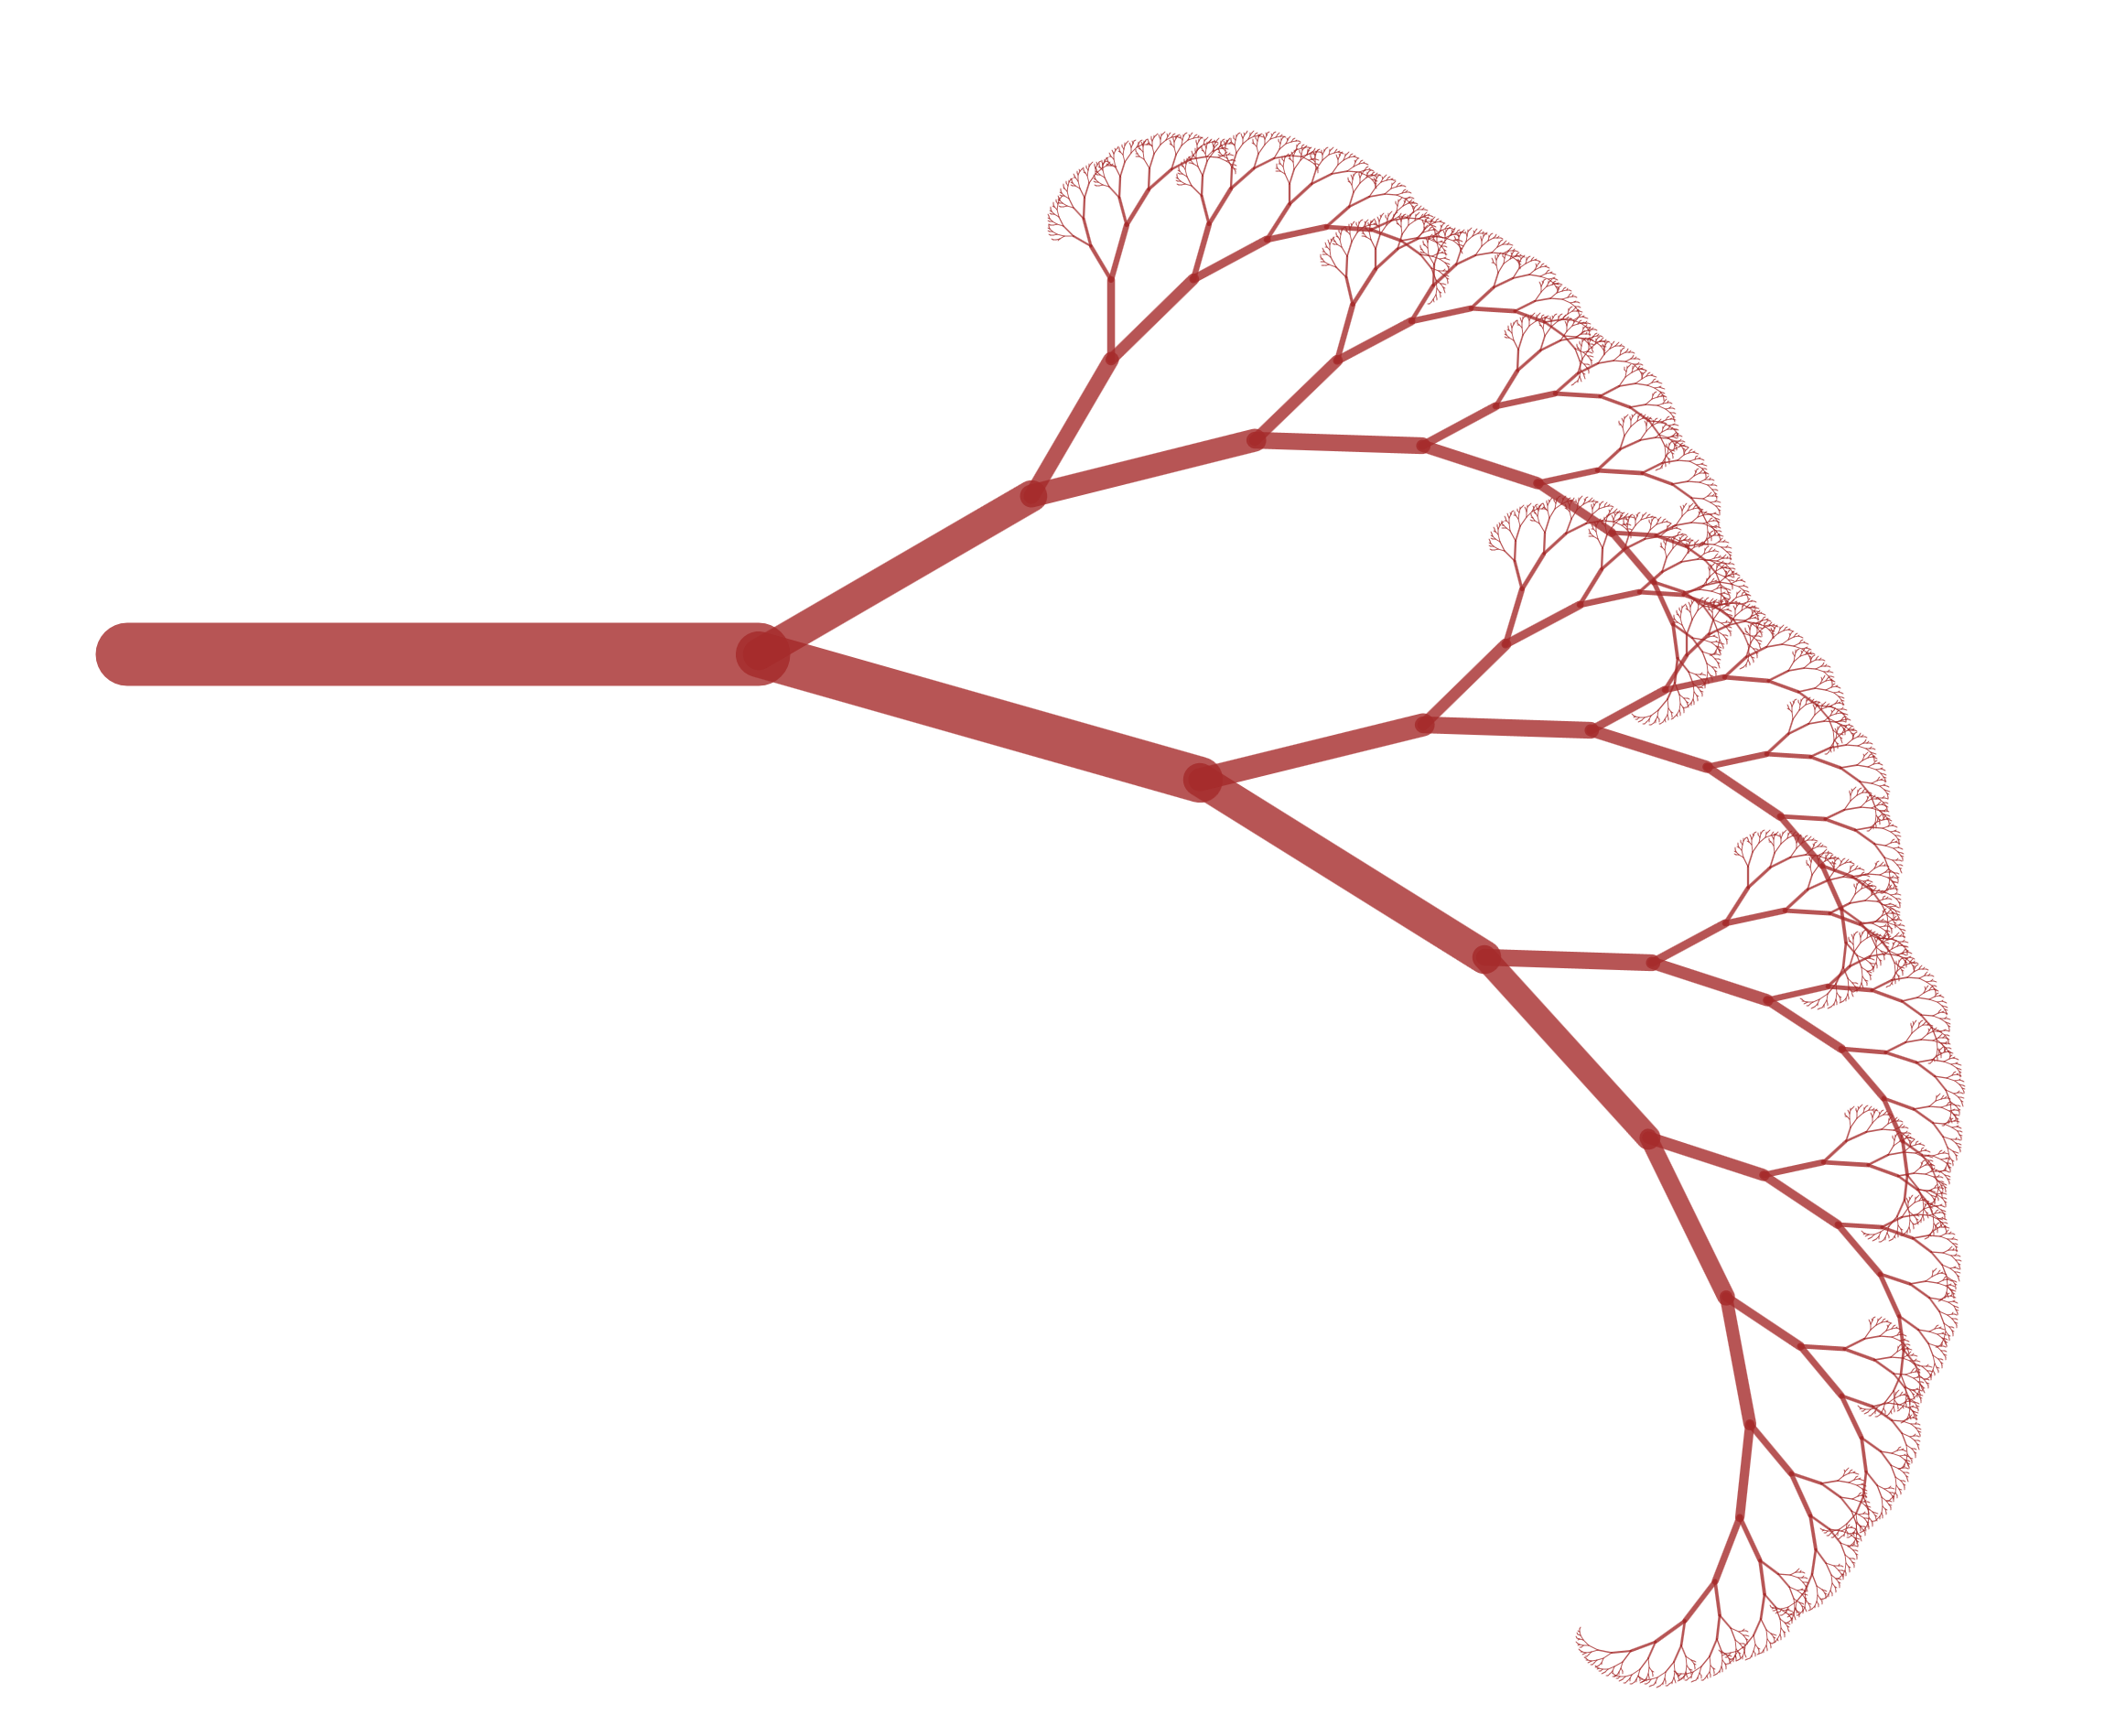
\includegraphics[width=0.8\textwidth]{img/simple03.png}
        \end{figure}

        \FloatBarrier

        Suppose then, that one would like to define several such functions, and combine them together.
        In order to accomplish that, there should be a way to tell apart different kinds of segments.
        A very straightforward method would be to give each segment a different color.
        In such a situation the previous example would translate to this (Figure~\ref{med01}).

        \begin{figure}[ht]
            \caption{\label{med01} Different Colors}
            \centering
            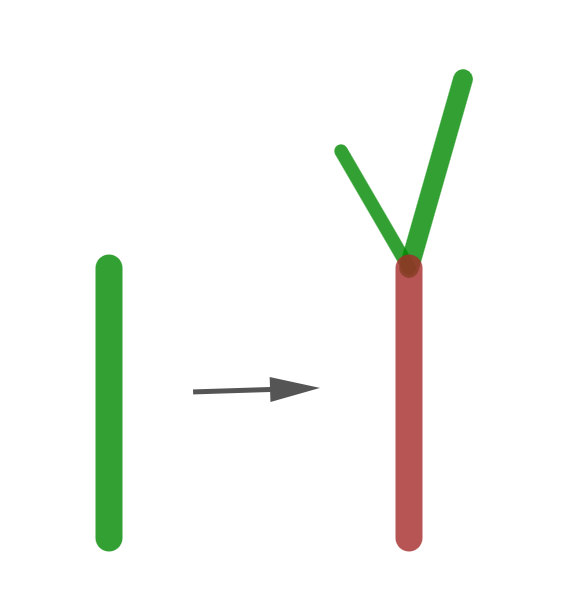
\includegraphics[width=0.16\textwidth]{img/med01.png}
        \end{figure}

        \FloatBarrier

        In this case the red segments will remain a simple segment while the green ones will transform further.
        Of course, it would be much clear if I would use arrows instead of simple segments because it might not be clear in which direction the segment should transform. 
        This will be discussed further in the paper.

        The fact that we use different colors allows not only to define a transformation in a much clear way, it also allows to implement much more interesting cases.
        Suppose that we have two functions defined in the following way.

        \begin{figure}[ht]
            \caption{\label{med02} Two transformation}
            \centering
            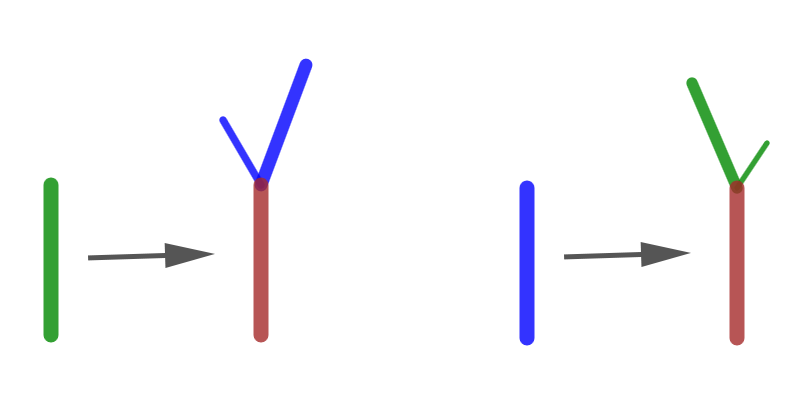
\includegraphics[width=0.4\textwidth]{img/med02.png}
        \end{figure}

        \FloatBarrier

        As one can see (Figure~\ref{med03}), this produces a fractal that is surprisingly similar to a real tree, even though the rules used are fairly simple.
        If we start with the blue segment instead of the green one, we get a slightly different tree, Figure~\ref{med04}.

        \begin{figure}[ht]
            \caption{\label{med03} A simple fractal tree.}
            \centering
            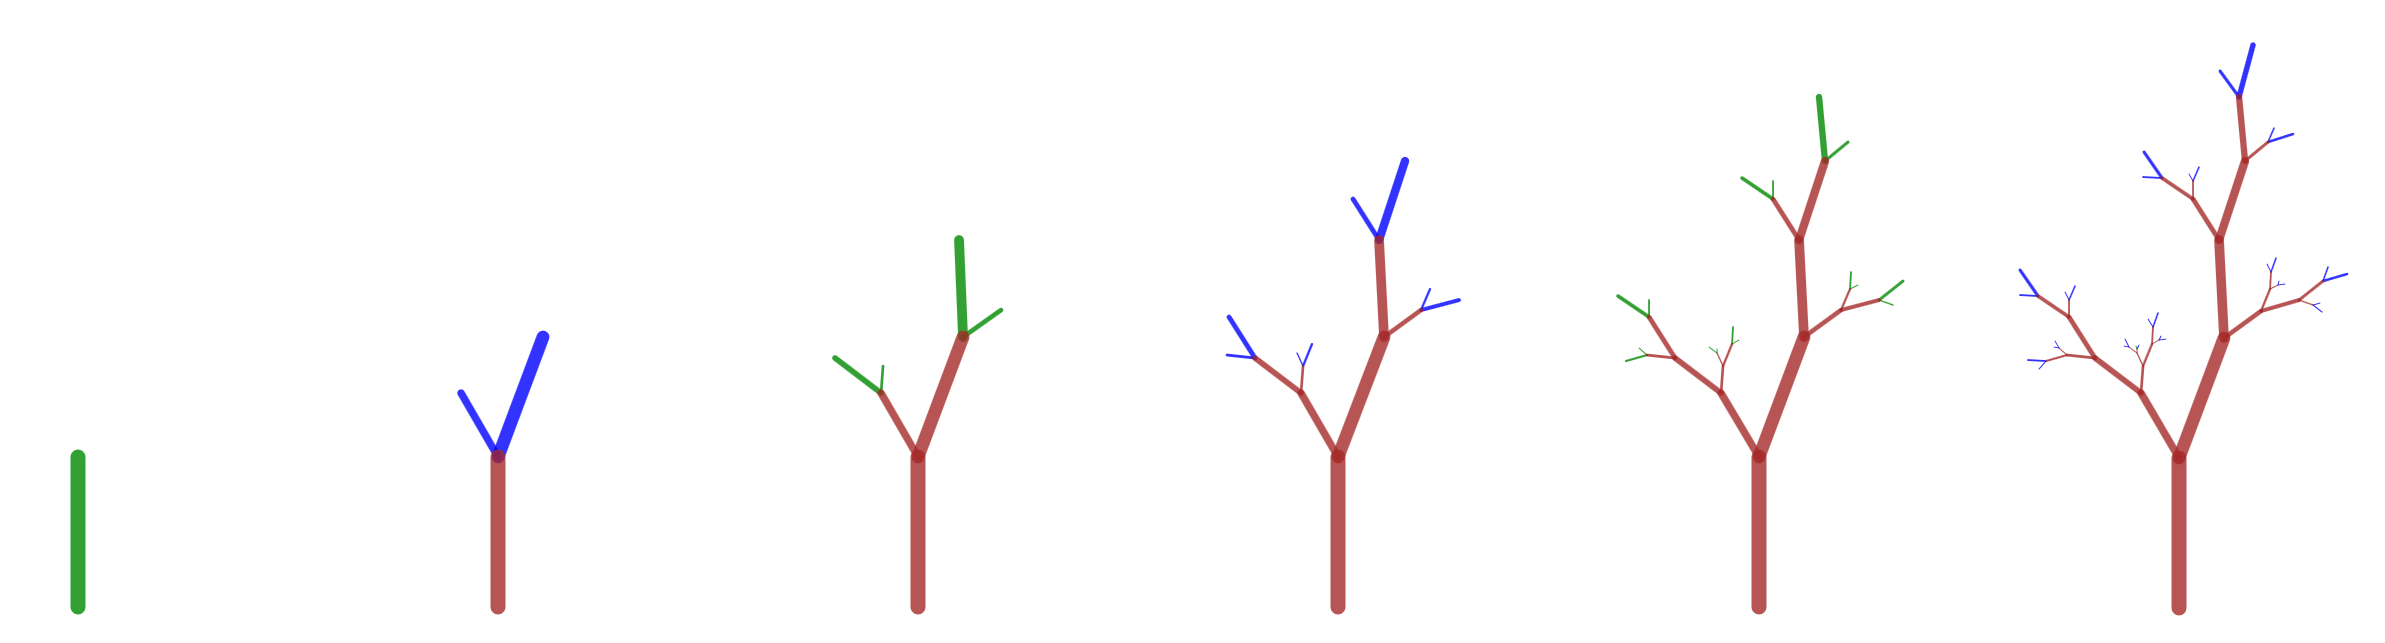
\includegraphics[width=0.9\textwidth]{img/med03.png}
        \end{figure}

        \begin{figure}[ht]
            \caption{\label{med04} Another simple fractal tree.}
            \centering
            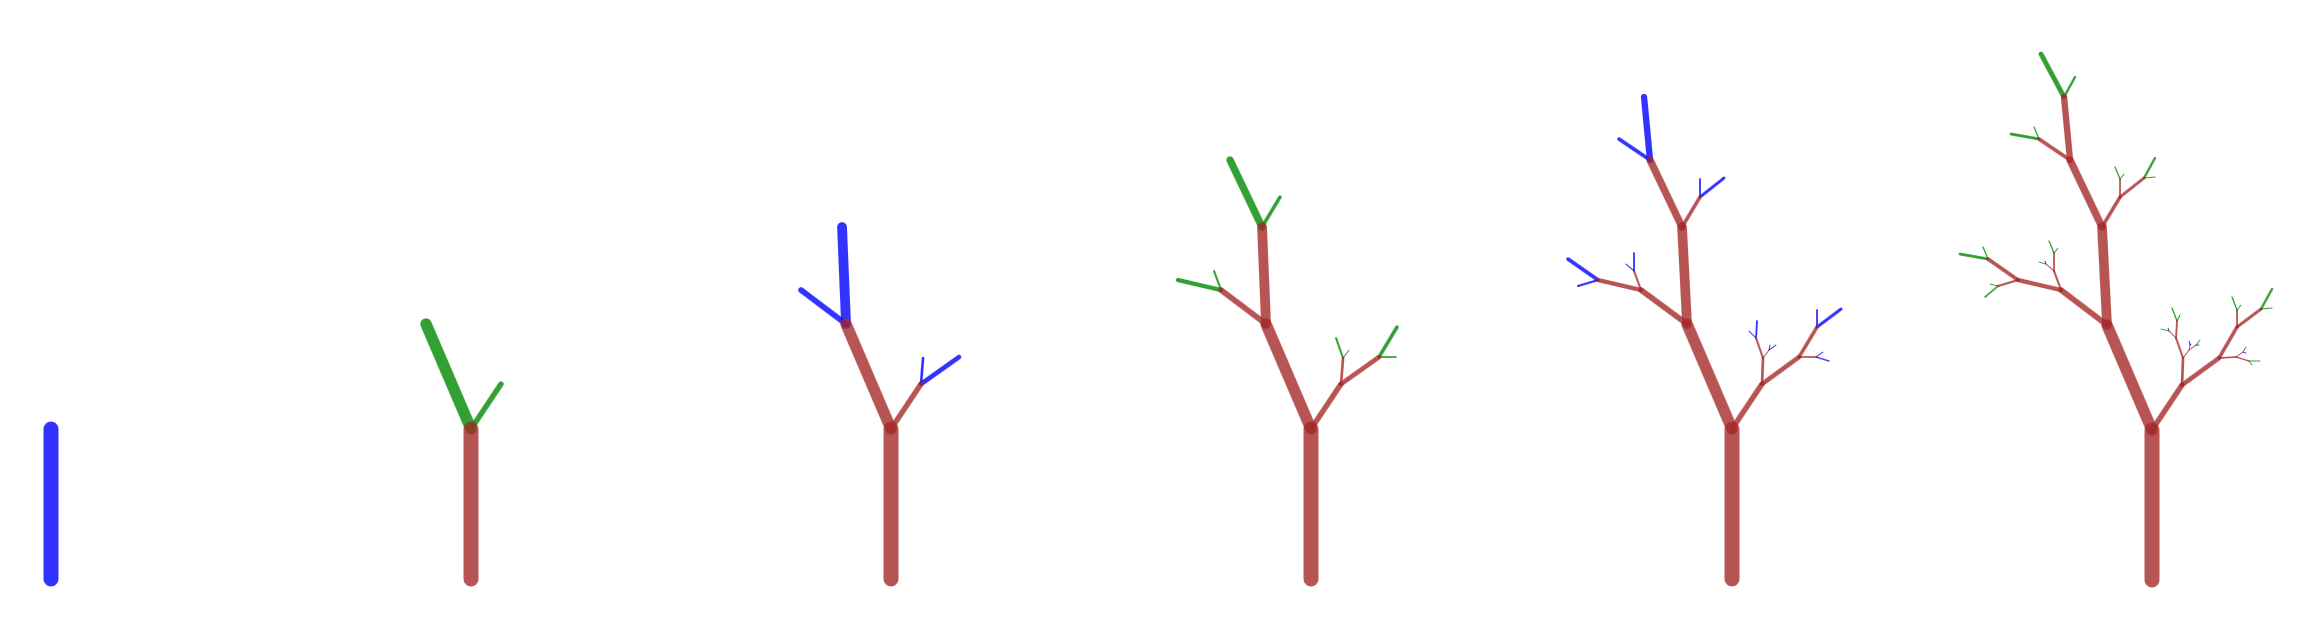
\includegraphics[width=0.9\textwidth]{img/med04.png}
        \end{figure}

        Figure~\ref{med05} shows the fractals in bigger detail.

        \begin{figure}[ht]
            \caption{\label{med05} Detailed Trees.}
            \centering
            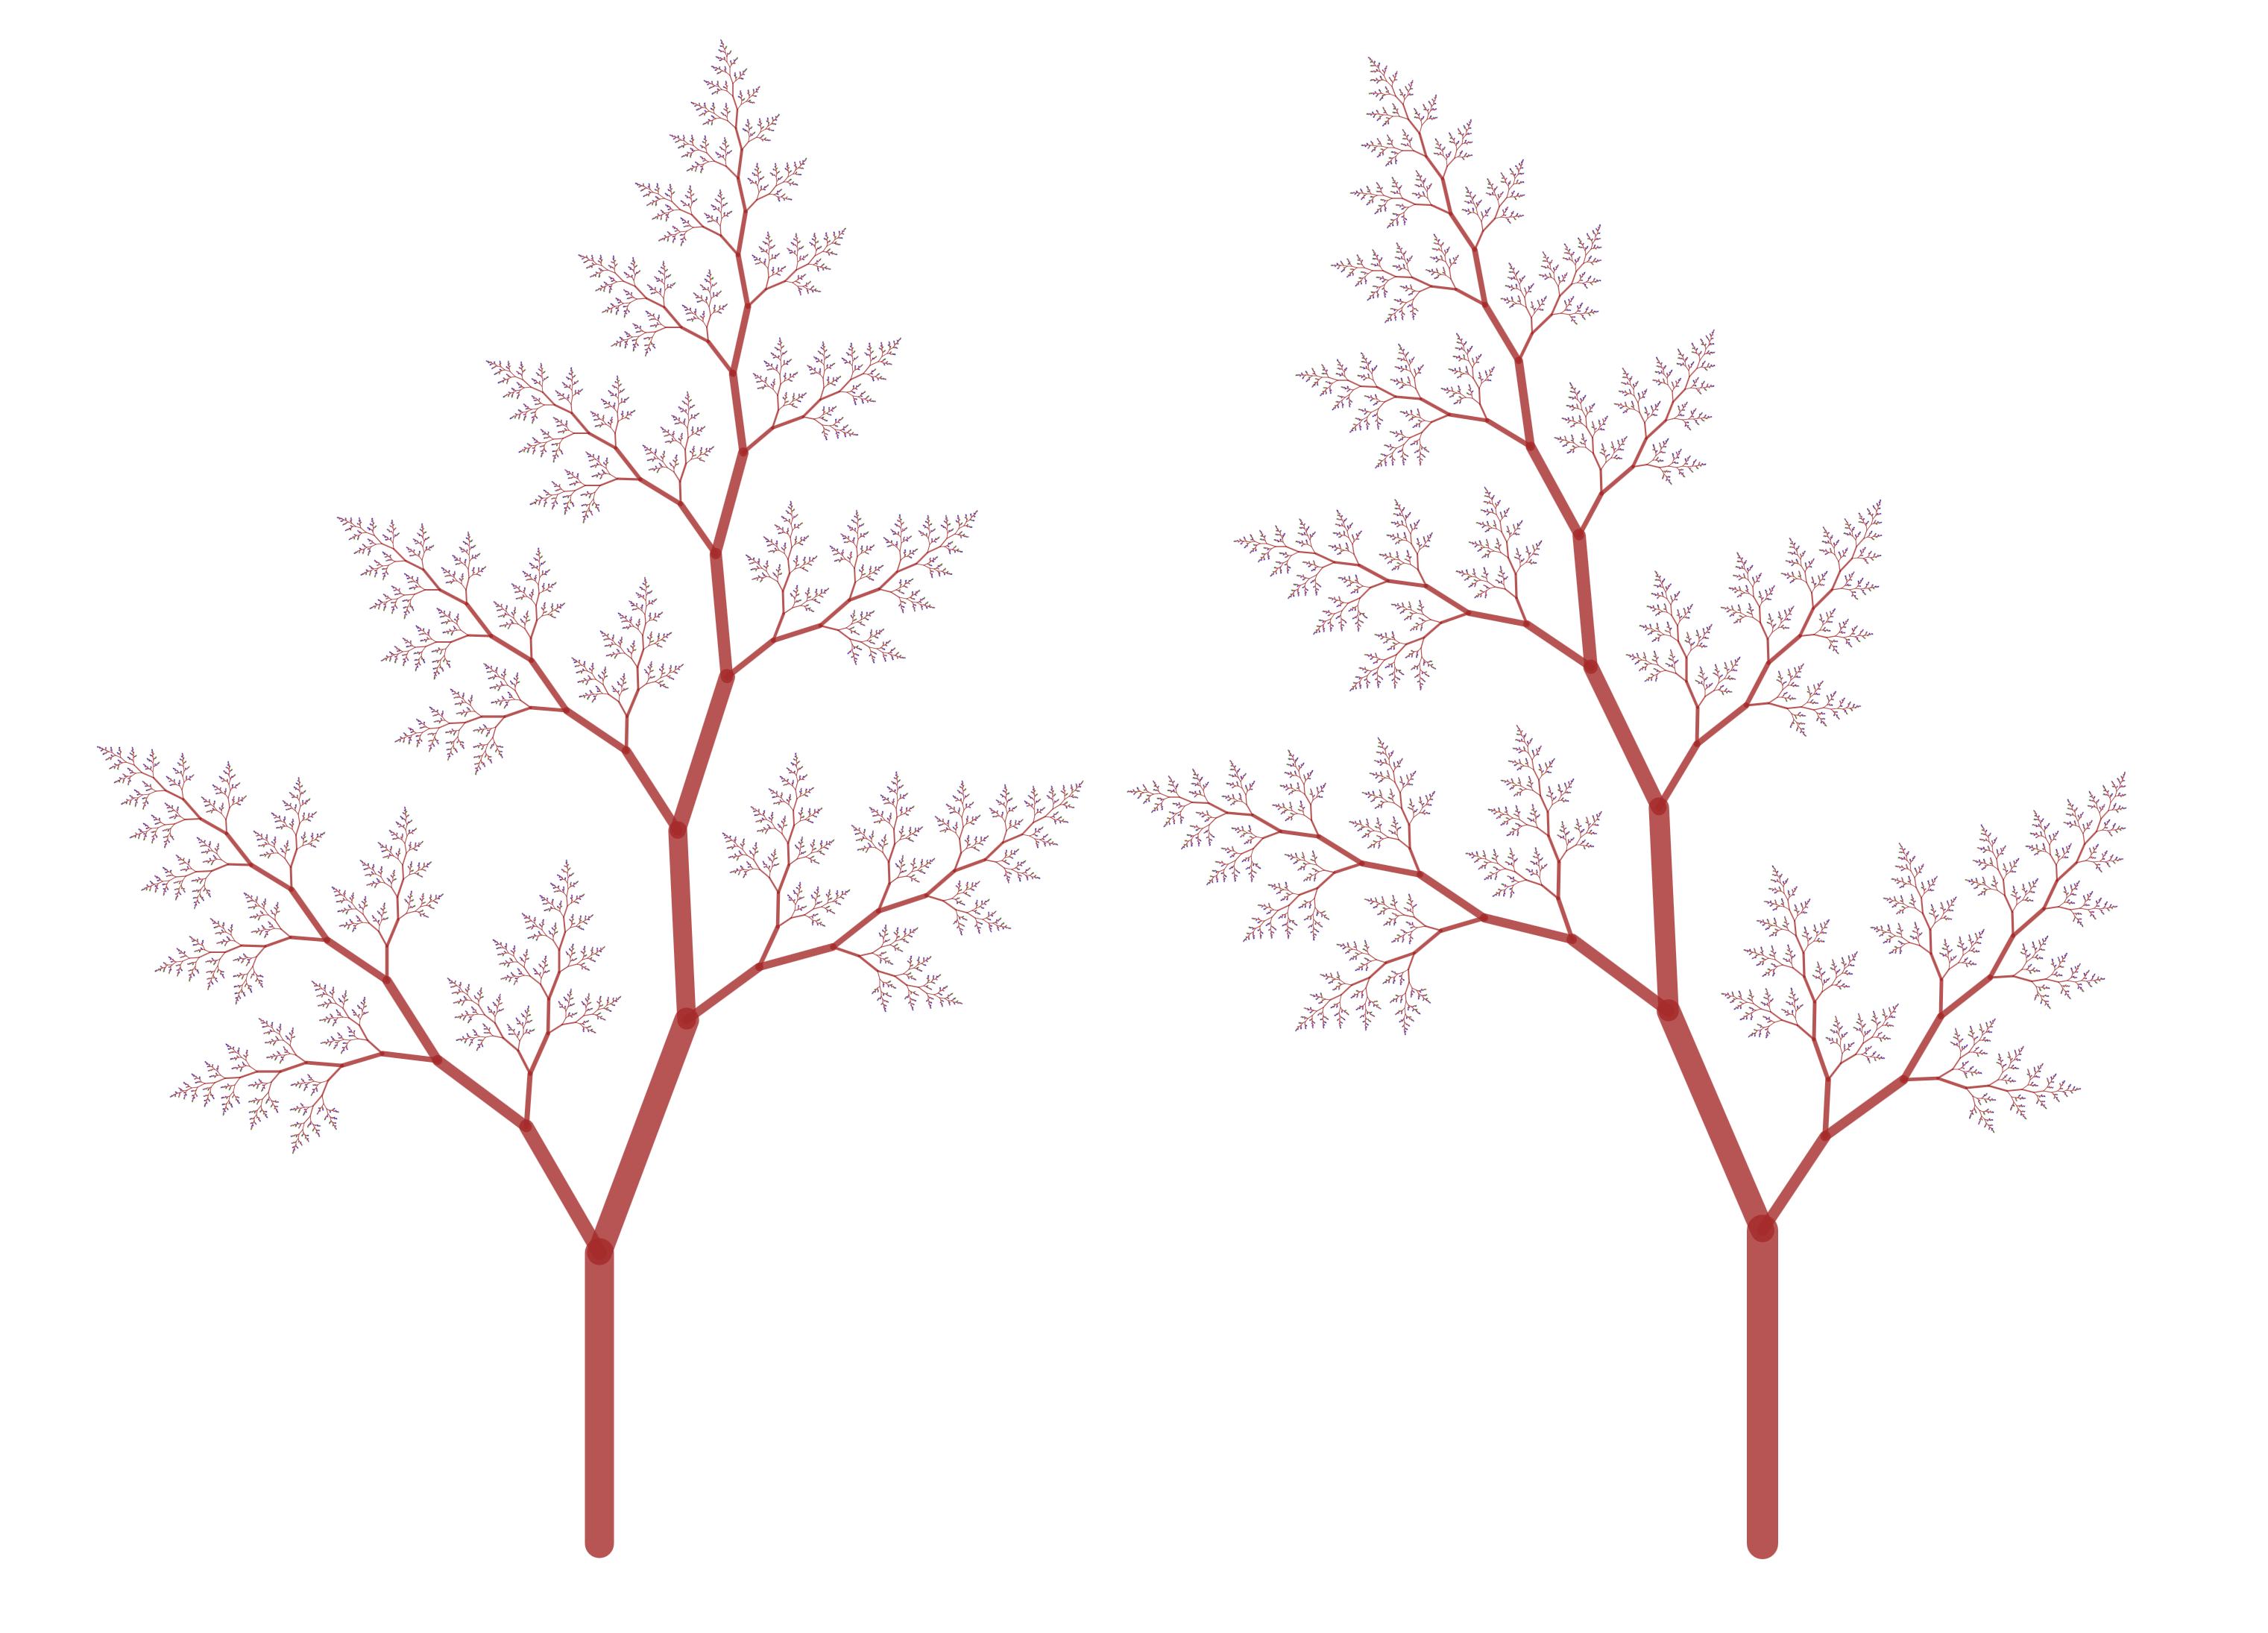
\includegraphics[width=\textwidth]{img/med05.png}
        \end{figure}

        \FloatBarrier

        At this moment, most of the readers might understand the basic idea of this project.
        In the next chapter I will try to explain how the GUI works and how the reader can create fractals by himself.

    \subsection{First steps}

        As I mentioned earlier, I started the work on the project with the idea that the program will be easy to use.
        There might exist other tools that allow the creation of iterated fractals, but most of them require advanced mathematical knowledge to understand and are a little cumbersome to use.

        \subsubsection{Basic controls}

            The way in which the user can create and manipulate a transformation is by dragging some circles.
            The circles can be dragged around by pressing and moving the \emph{left mouse button}.
            To create a new circle a user can press the \emph{right mouse button} on the background.
            To delete a circle the user should click the \emph{middle mouse button}.

            To create and arrow, one should drag a circle with the \emph{right mouse button}.
            To delete a segment, one should click the segment with the \emph{middle mouse button}.
            To change the type of the segment, one should click the segment with the \emph{left mouse button}.

            The concept are this: 
            \begin{enumerate}
                \item left button = move/change
                \item right button = create
                \item middle button = delete
            \end{enumerate}
            These were all the basic instructions. 
            Knowing how to use them is enough to create and edit a segment transformation.

        \subsubsection{The base layer and simple layers}

            A transformation can be create inside a layer. 
            A new layer can be create by pressing the \emph{Add Layer} button.
            Figure~\ref{gui01} shows how a new layer looks.

            \begin{figure}[ht]
                \caption{\label{gui01} A new layer.}
                \centering
                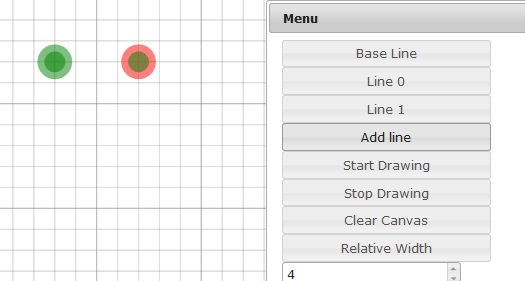
\includegraphics[width=0.5\textwidth]{img/gui01.png}
            \end{figure}

            The inner color of the circles represents the color of the transformation.
            The outer color represents the type of specific circles inside a layer.
            The circle with the outer color green is the start point and the circle with the outer color red is the end point.

            Lets try to implement the tree showed previously.
            First lets move the circles so that they stand vertically and also add two circles by pressing the \emph{right mouse button} on the background.

            \begin{figure}[ht]
                \centering
                \caption{Points and segments.}
                \subcaptionbox{\label{gui02} Two new points.}[.4\linewidth]
                    {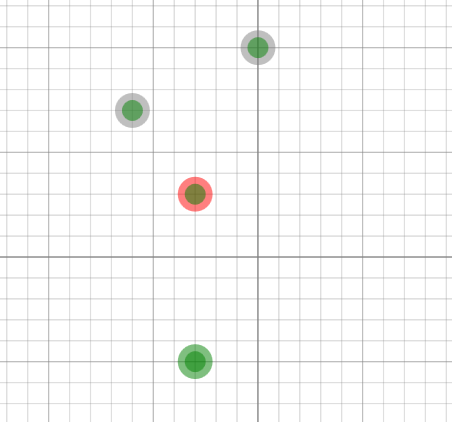
\includegraphics[height=0.35\textwidth]{img/gui02.png}}
                \subcaptionbox{\label{gui03} The first segments.}[.4\linewidth]
                    {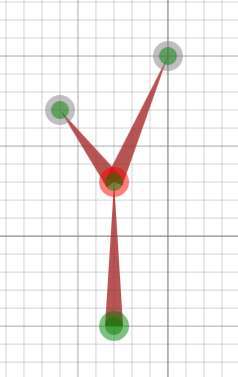
\includegraphics[height=0.35\textwidth]{img/gui03.png}}

            \end{figure}

            In order to create a segment the user should drag from a disk to another using the right mouse button (Figure~\ref{gui03}).

            \FloatBarrier

            It can be observed that all the arrows have the same color, red (it could be any other color). 
            But we didn't define a red type of transformation, so were do we have it.


        \subsubsection{Identity Layer}

            If we'll switch to Layer 0 by clicking the appropriate button we will see this (Fig.~\ref{identity01}).
            You can observe that the inner color of the circles is different, that's because we switched to a different layer.

            \begin{figure}[ht]
                \caption{\label{identity01} The identity layer.}
                \centering
                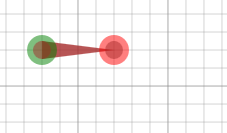
\includegraphics[width=0.3\textwidth]{img/identity01.png}
            \end{figure}

            The identity layer is a little bit different from other layers.
            First of all, even though we can drag the circles around, we cannot add more circles or change the type of the arrow.

            \FloatBarrier

            The identity layer draws itself, that is, it does not transform to something different.
            Because of this property, there are some optimizations that can be implemented.
            For example instead of recursing further when finding a identity layer, the program will just draw the line because it can infer that 
            the segment will not transform to something different.

            Coming back to Layer 1, we can click each of the upper arrows in order to change their colors (Fig.~\ref{gui04}).

            \begin{figure}[ht]
                \caption{\label{gui04} Different types of arrows.}
                \centering
                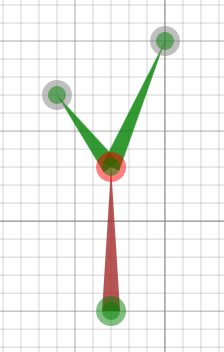
\includegraphics[width=0.2\textwidth]{img/gui04.png}
            \end{figure}
            \FloatBarrier

            The new color is green, that is, the color of the current layer.
            If we would click the arrows one more time they would, once again, change their color to the color of the identity layer.

            Even though we basically define all that is required we don't see anything happening.

        \subsubsection{The Base Layer}

            The uppermost Layer (Fig.~\ref{baselayer01}), called the base layer is different from all the other layers.
            First of all it does not have a initial green and red circle. 

            \begin{figure}[ht]
                \caption{\label{baselayer01} The Base Layer.}
                \centering
                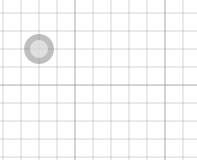
\includegraphics[width=0.2\textwidth]{img/baselayer01.png}
            \end{figure}

            The base layer is used not to define a transformation but to apply them.
            Lets create another point and connect these two points with an arrow.

            \begin{figure}[H]
                \centering
                \caption{Changing the color of the arrow.}
                \subcaptionbox{\label{baselayer02} First try.}[0.4\textwidth]
                    {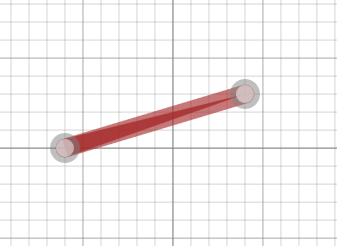
\includegraphics[width=0.3\textwidth]{img/baselayer02.png}}
                ~
                \subcaptionbox{\label{baselayer03} Second try.}[0.5\textwidth]
                    {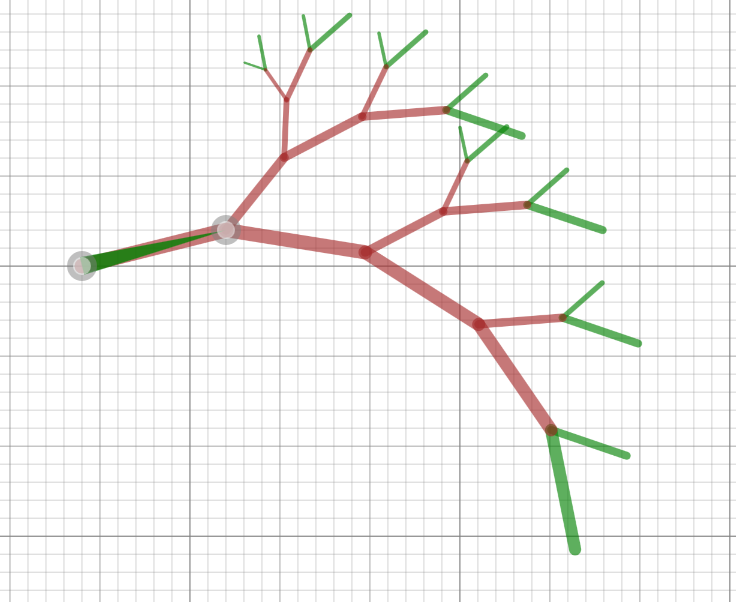
\includegraphics[width=0.45\textwidth]{img/baselayer03.png}}
            \end{figure}

            Something interesting happens. 
            Just as we connected the circles, an thick arrow appeared on the background.
            Because the arrow is of identity type it just created a line.
            Lets try to press the arrow in order to change the type.

            \FloatBarrier

            Figure~\ref{baselayer03} shows that we created our first, own fractal tree.
            If we move the circles around the tree will move along.
            This is because the \emph{Dynamic Drawing} check-box is on, we'll talk about this feature later.

            Another interesting feature is that if we switch to Layer 1 and move the circles there, the tree will also change (Fig.~\ref{baselayer04}).
            It is important to not get confused at this point.
            For some it might be strange that the the root of the tree does not coincide with the identity arrow in Layer 1.
            This is because Layer are used to define transformation that are applied to the Base Layer.
            Only the Base Layer defines the position of the initial segments.

            \begin{figure}[ht]
                \caption{\label{baselayer04} Perspective from another layer.}
                \centering
                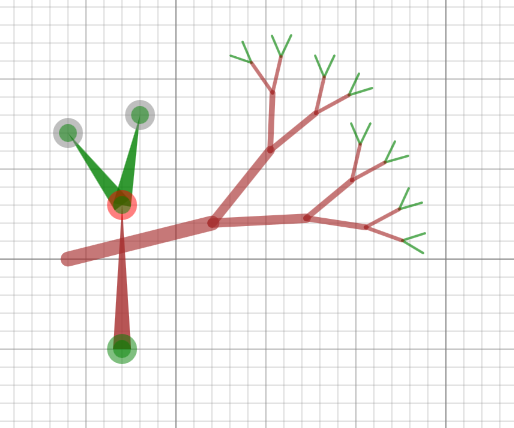
\includegraphics[width=0.3\textwidth]{img/baselayer04.png}
            \end{figure}

    \subsection{Common fractals}

        During this and the subsequent chapters I will show some fractals and other geometric structures that can be created using this soft.
        Also, in this way I will try to give some insight and useful information about the GUI.
        I think that a hands-on approach would be much more insightful than any other method of explanation.

        \subsubsection{The Dragon Curve}

            The Dragon Curve is very easy to create.
            This setup (Fig.~\ref{dragon01}) is required in a new layer.

            \begin{figure}[ht]
                \caption{The Dragon Curve.}
                \centering
                \subcaptionbox{\label{dragon01} The setup.}[0.3\textwidth]
                    {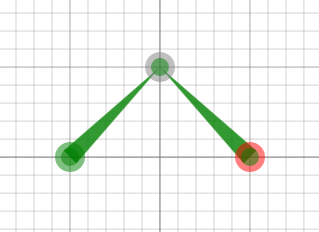
\includegraphics[width=0.3\textwidth]{img/dragon01.png}}
                ~
                \subcaptionbox{\label{dragon02} Dragon Curve after 4 steps.}[0.3\textwidth]
                    {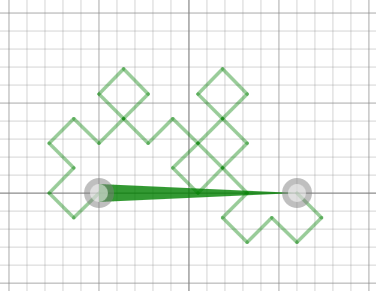
\includegraphics[width=0.3\textwidth]{img/dragon02.png}}
            \end{figure}

            Adding a arrow in the base layer we get this (Fig.~\ref{dragon02}).

            To increase the recursion level the user must use the spinner in the main dialog.
            This is what can be created (Fig.~\ref{dragon03}).

            \begin{figure}[ht]
                \caption{\label{dragon03} The Dragon Curve.}
                \centering
                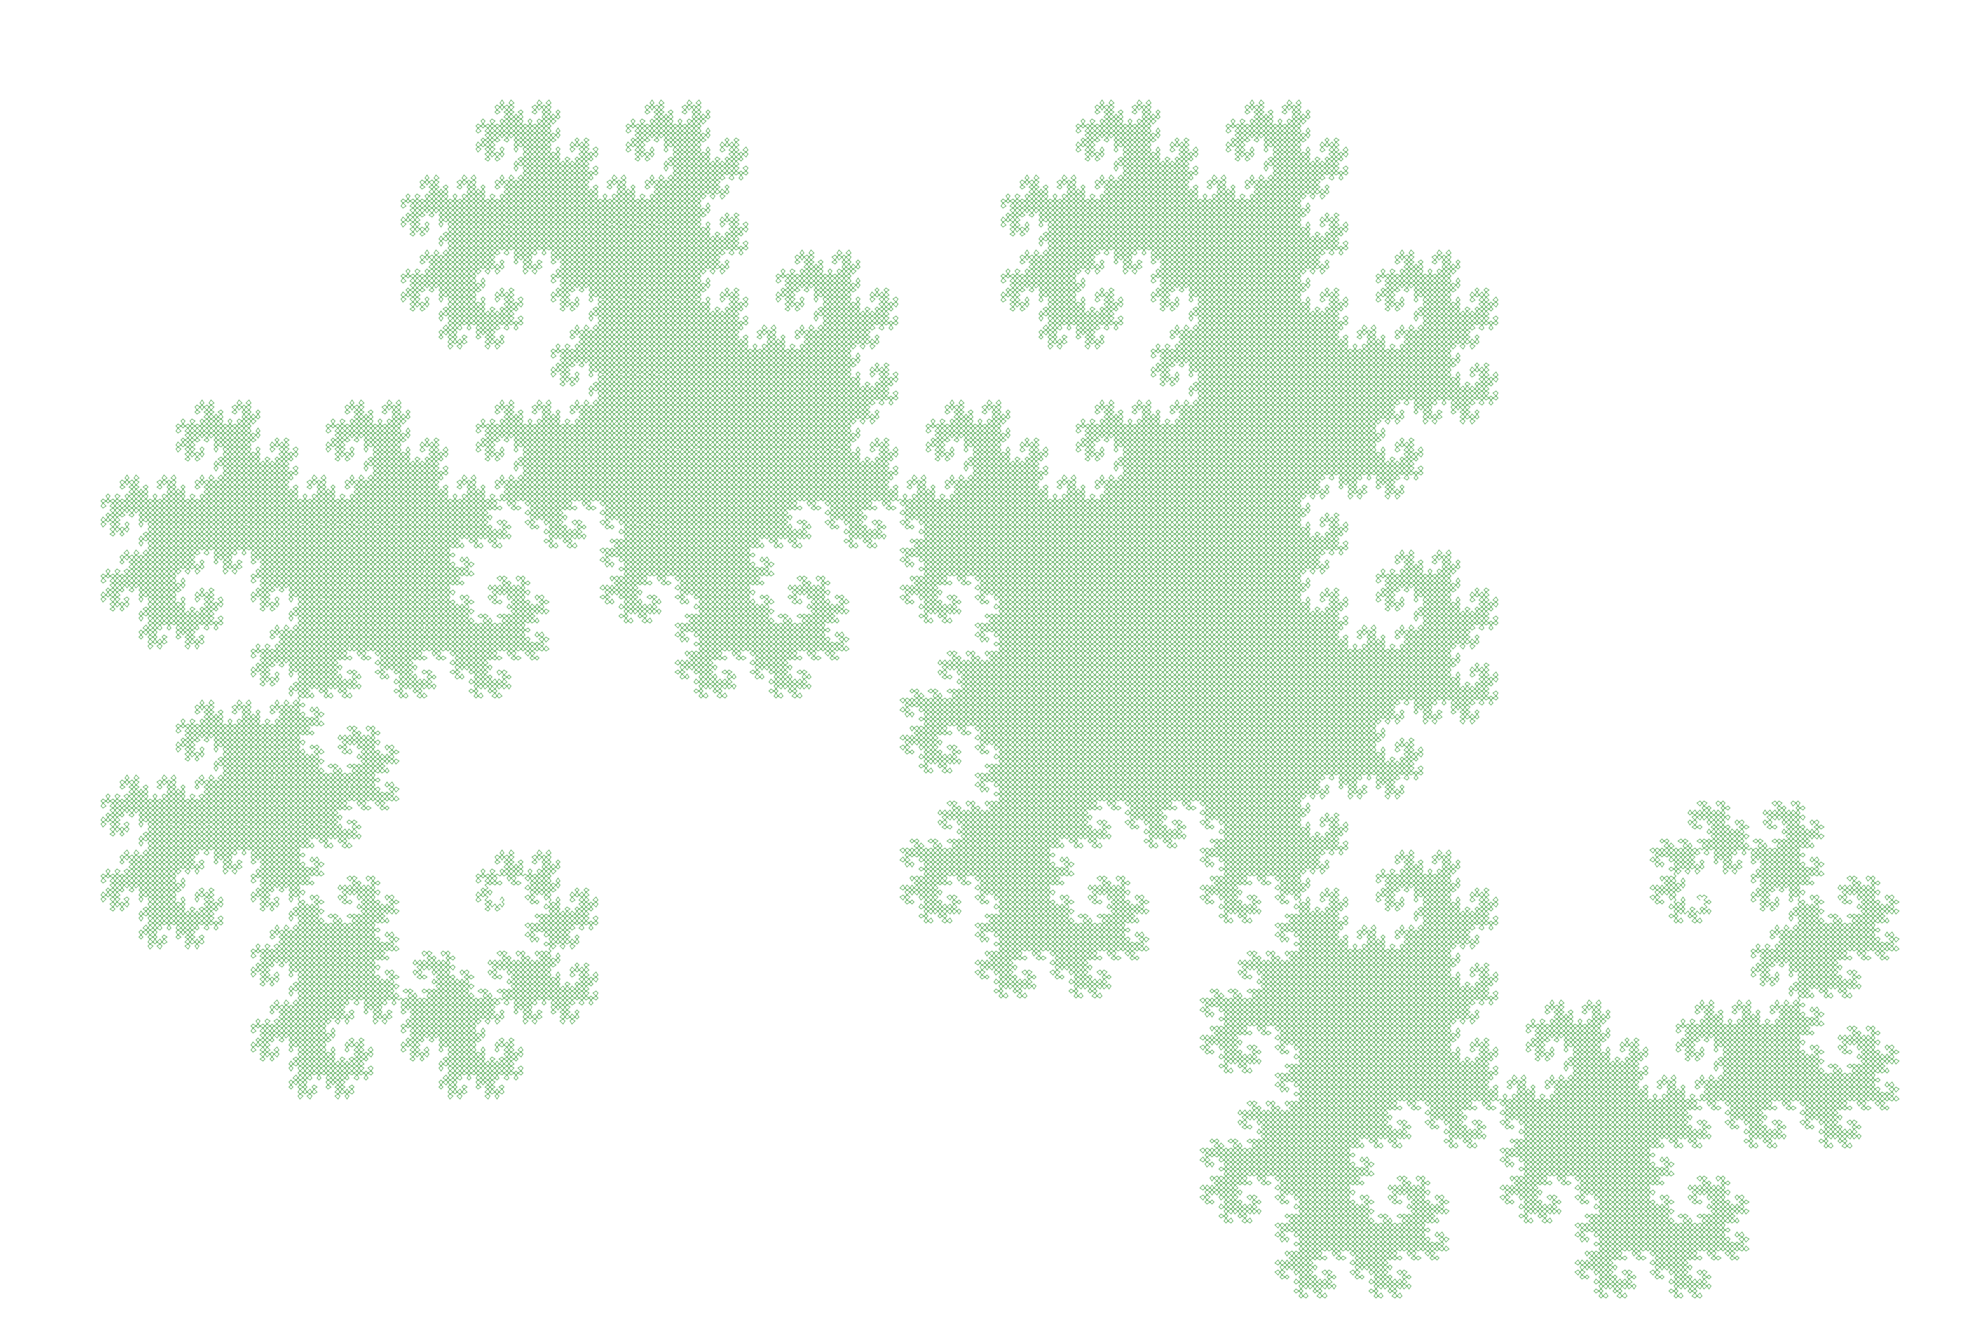
\includegraphics[width=0.96\textwidth]{img/dragon03.png}
            \end{figure}

            \FloatBarrier

        \subsubsection{Levy C Curve}

            The setup for the Levy C Curve is very similar to the Dragon Curve.
            
            \begin{figure}[ht]
                \caption{\label{levyc01} The setup.}
                \centering
                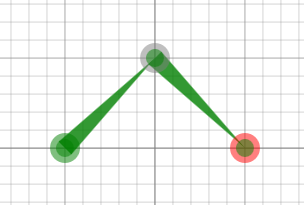
\includegraphics[width=0.3\textwidth]{img/levyc01.png}
            \end{figure}

            It is interesting that changing the direction of the arrow can have such an impact.

            \begin{figure}[ht]
                \caption{\label{levyc02} Levy C Curve.}
                \centering
                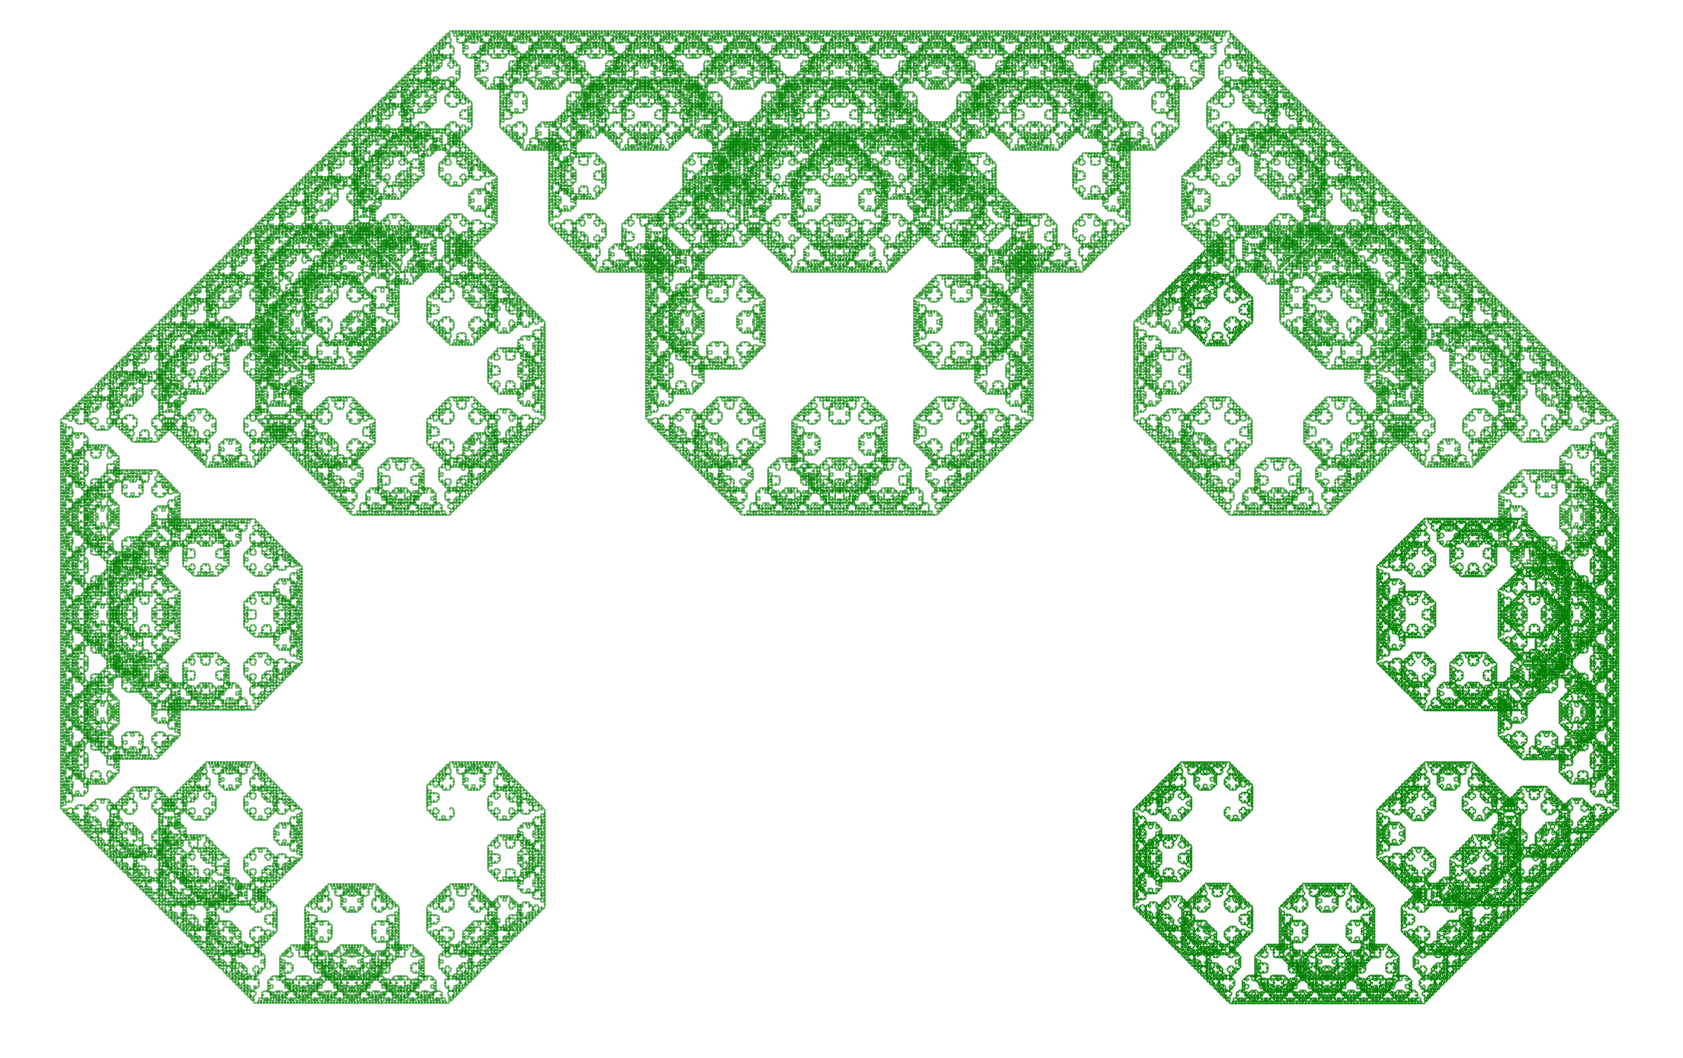
\includegraphics[width=0.9\textwidth]{img/levyc02.png}
            \end{figure}

            \FloatBarrier

        \subsubsection{Koch Snowflake and the Polar Grid}

            Lets try to create the Koch Snowflake.

            \begin{figure}[ht]
                \caption{Koch Snowflake.}
                \centering
                \begin{subfigure}[b]{0.49\textwidth}
                    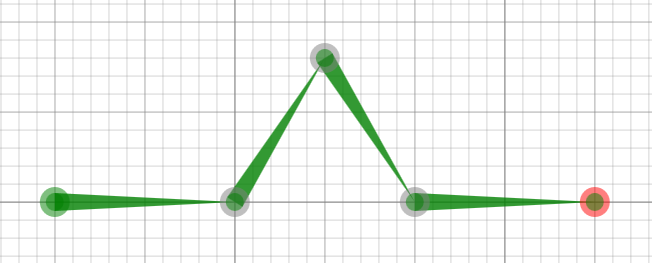
\includegraphics[width=\textwidth]{img/snowflake_setup.png}
                    \caption{Cartesian grid \label{snowflake_setup}}
                \end{subfigure}
                ~
                \begin{subfigure}[b]{0.49\textwidth}
                    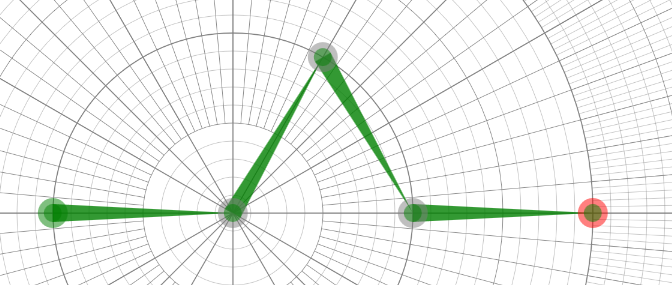
\includegraphics[width=\textwidth]{img/snowflake_setup02.png}
                    \caption{Polar grid \label{snowflake_setup_02}}
                \end{subfigure}
            \end{figure}

            The problem, as one can see, is that it is basically impossible to create an angle of 60 degrees using the cartesian coordinates.
            To solve this problem I came up with an interesting idea.
            I implemented a polar grid.
            To switch to it the user has to press the \emph{Polar Grid} button.
            The center of the polar grid will be \emph{the last pressed circle}.
            Below is the new setup.

            The setup in the Base Layer can be the following (Fig.~\ref{snowflake_setup03}).

            \begin{figure}[ht]
                \caption{\label{snowflake_setup03} Base Layer setup.}
                \centering
                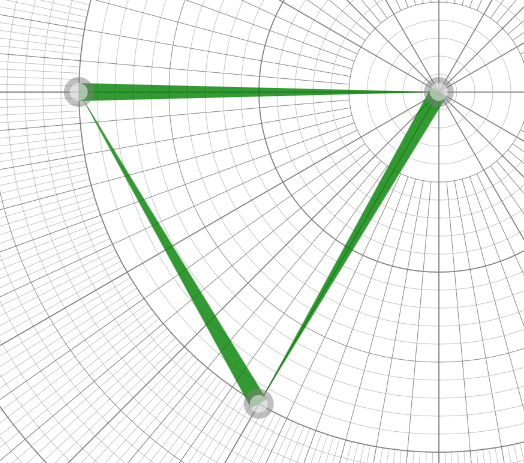
\includegraphics[width=0.3\textwidth]{img/snowflake_setup03.png}
            \end{figure}

            The drawing is in Figure~\ref{snowflake_draw}.

            \begin{figure}[ht]
                \caption{\label{snowflake_draw} Koch Snowflake.}
                \centering
                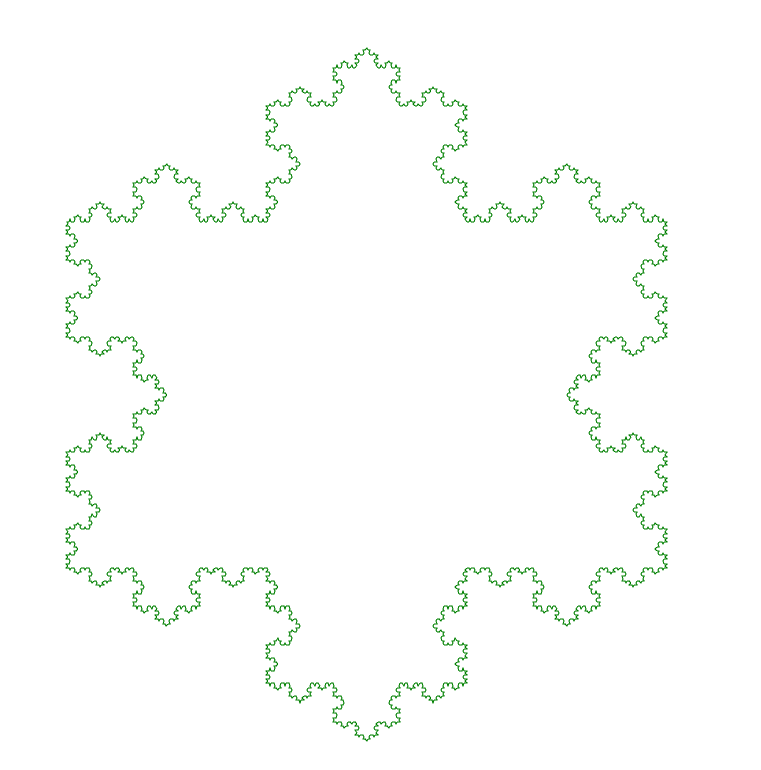
\includegraphics[width=0.6\textwidth]{img/snowflake_draw.png}
            \end{figure}

            \FloatBarrier

        \subsubsection{Some Quadratic curves}

            Following Koch's concept other types of curves were introduced.

            \begin{figure}[ht]
                \caption{\label{quadratic_01} Quadratic type 1.}
                \centering
                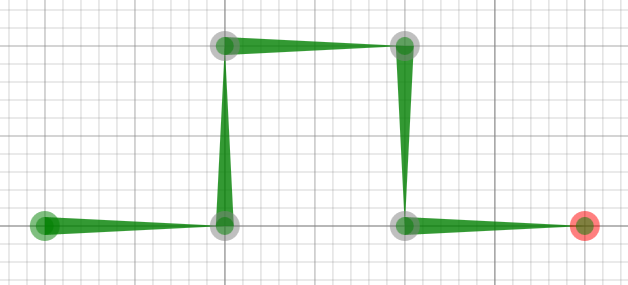
\includegraphics[width=0.3\textwidth]{img/quadratic_01setup.png}
                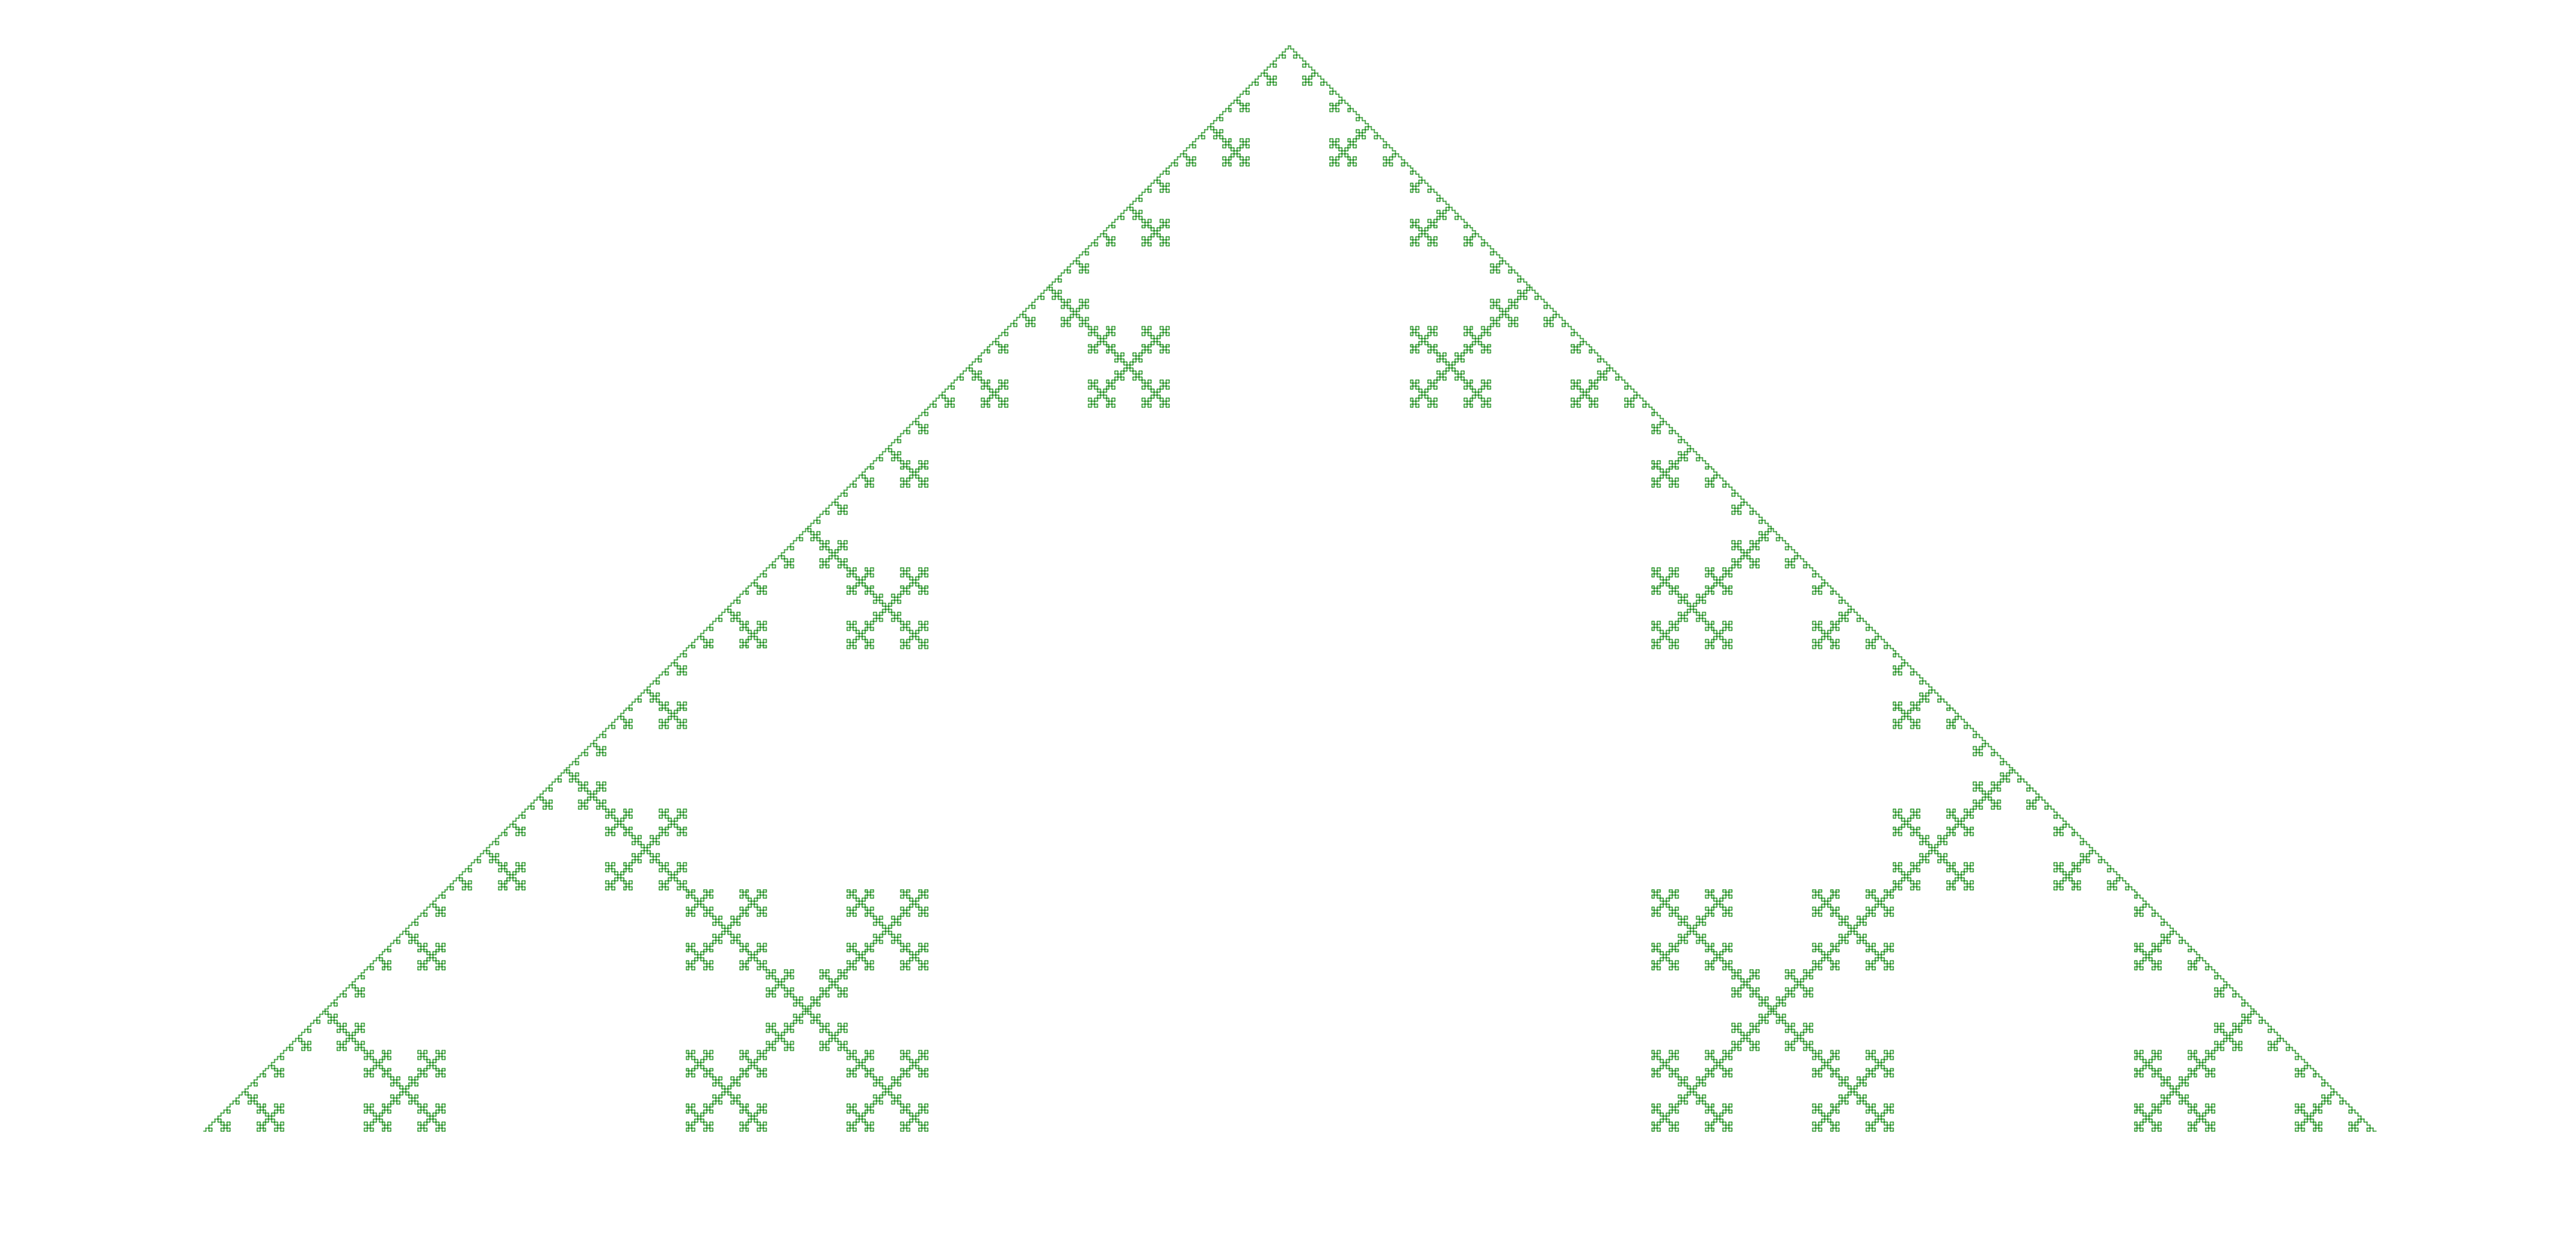
\includegraphics[width=0.67\textwidth]{img/quadratic_01draw.png}
            \end{figure}

            \begin{figure}[ht]
                \caption{\label{quadratic_02} Quadratic type 2.}
                \centering
                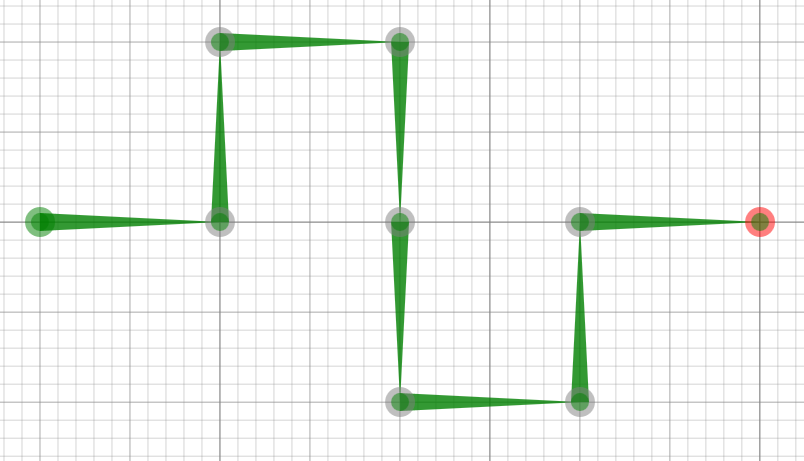
\includegraphics[width=0.3\textwidth]{img/quadratic_02setup.png}
                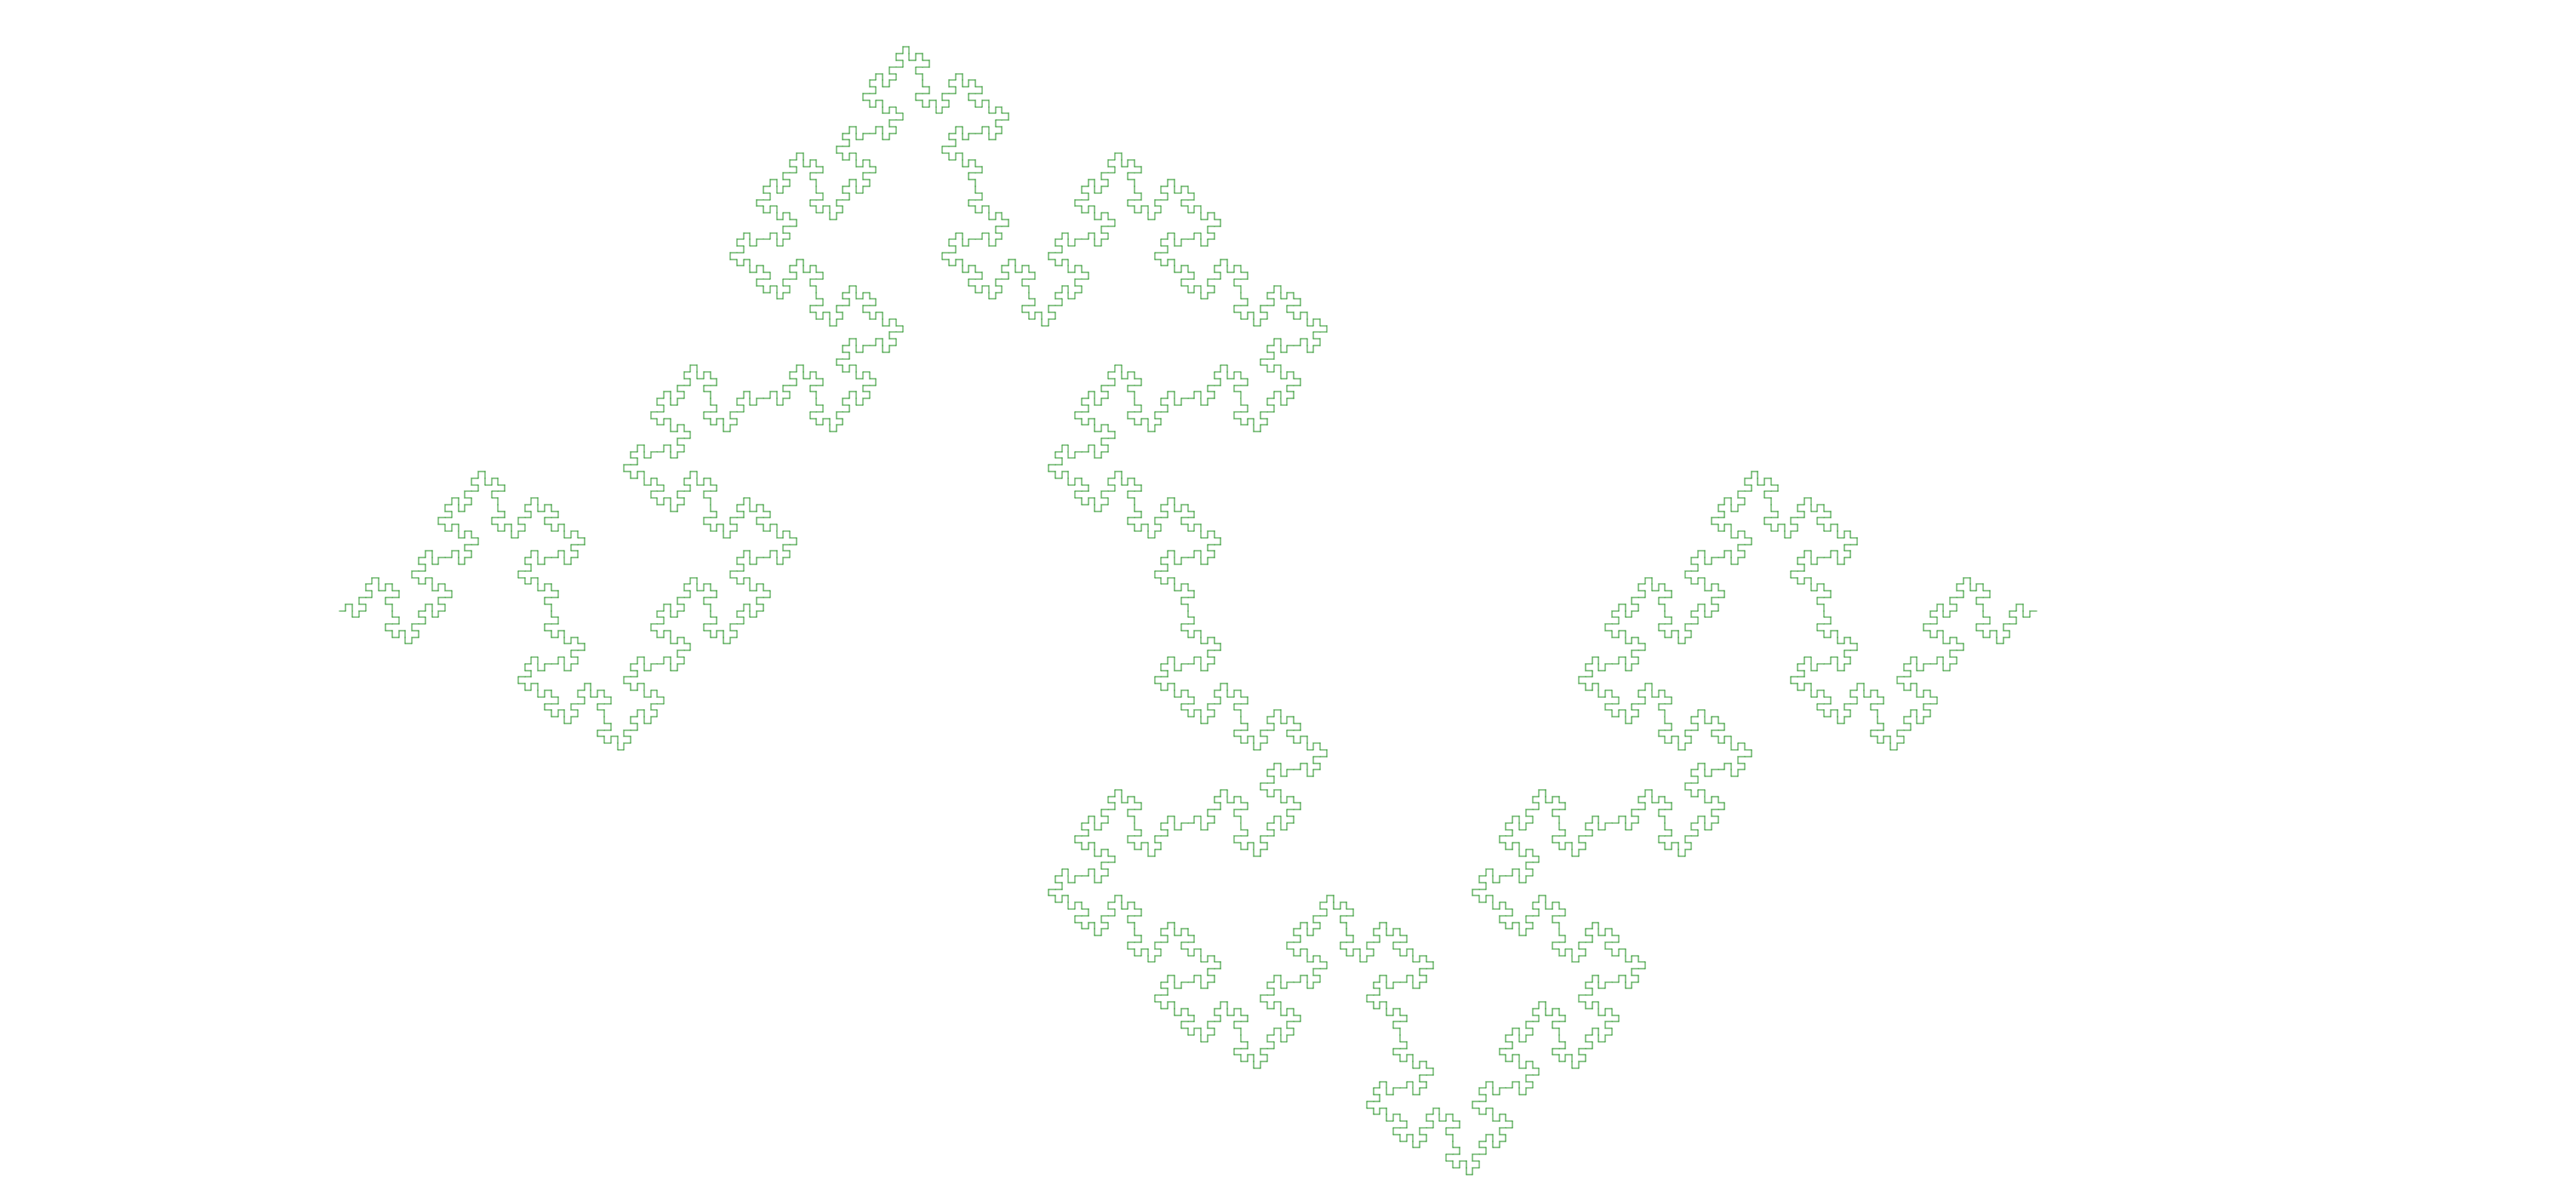
\includegraphics[width=0.67\textwidth]{img/quadratic_02draw.png}
            \end{figure}

            \FloatBarrier

        \subsubsection{Variations}

            At this moment it will probably be already clear that the program is not bound to create rigorously defined fractals. 
            The user can choose to create a lot of different variations with ease.
            The fact that the lines are drawn dynamically make this even more interesting.
            The pictures in Figure \ref{koch_variatinos_01} show just a very few of the types of Koch curve variations that can be created.
            I will come back to Koch variations in later chapter.

            \begin{figure}[ht]
                \caption{\label{koch_variatinos_01} Koch Curve variations}
                \centering
                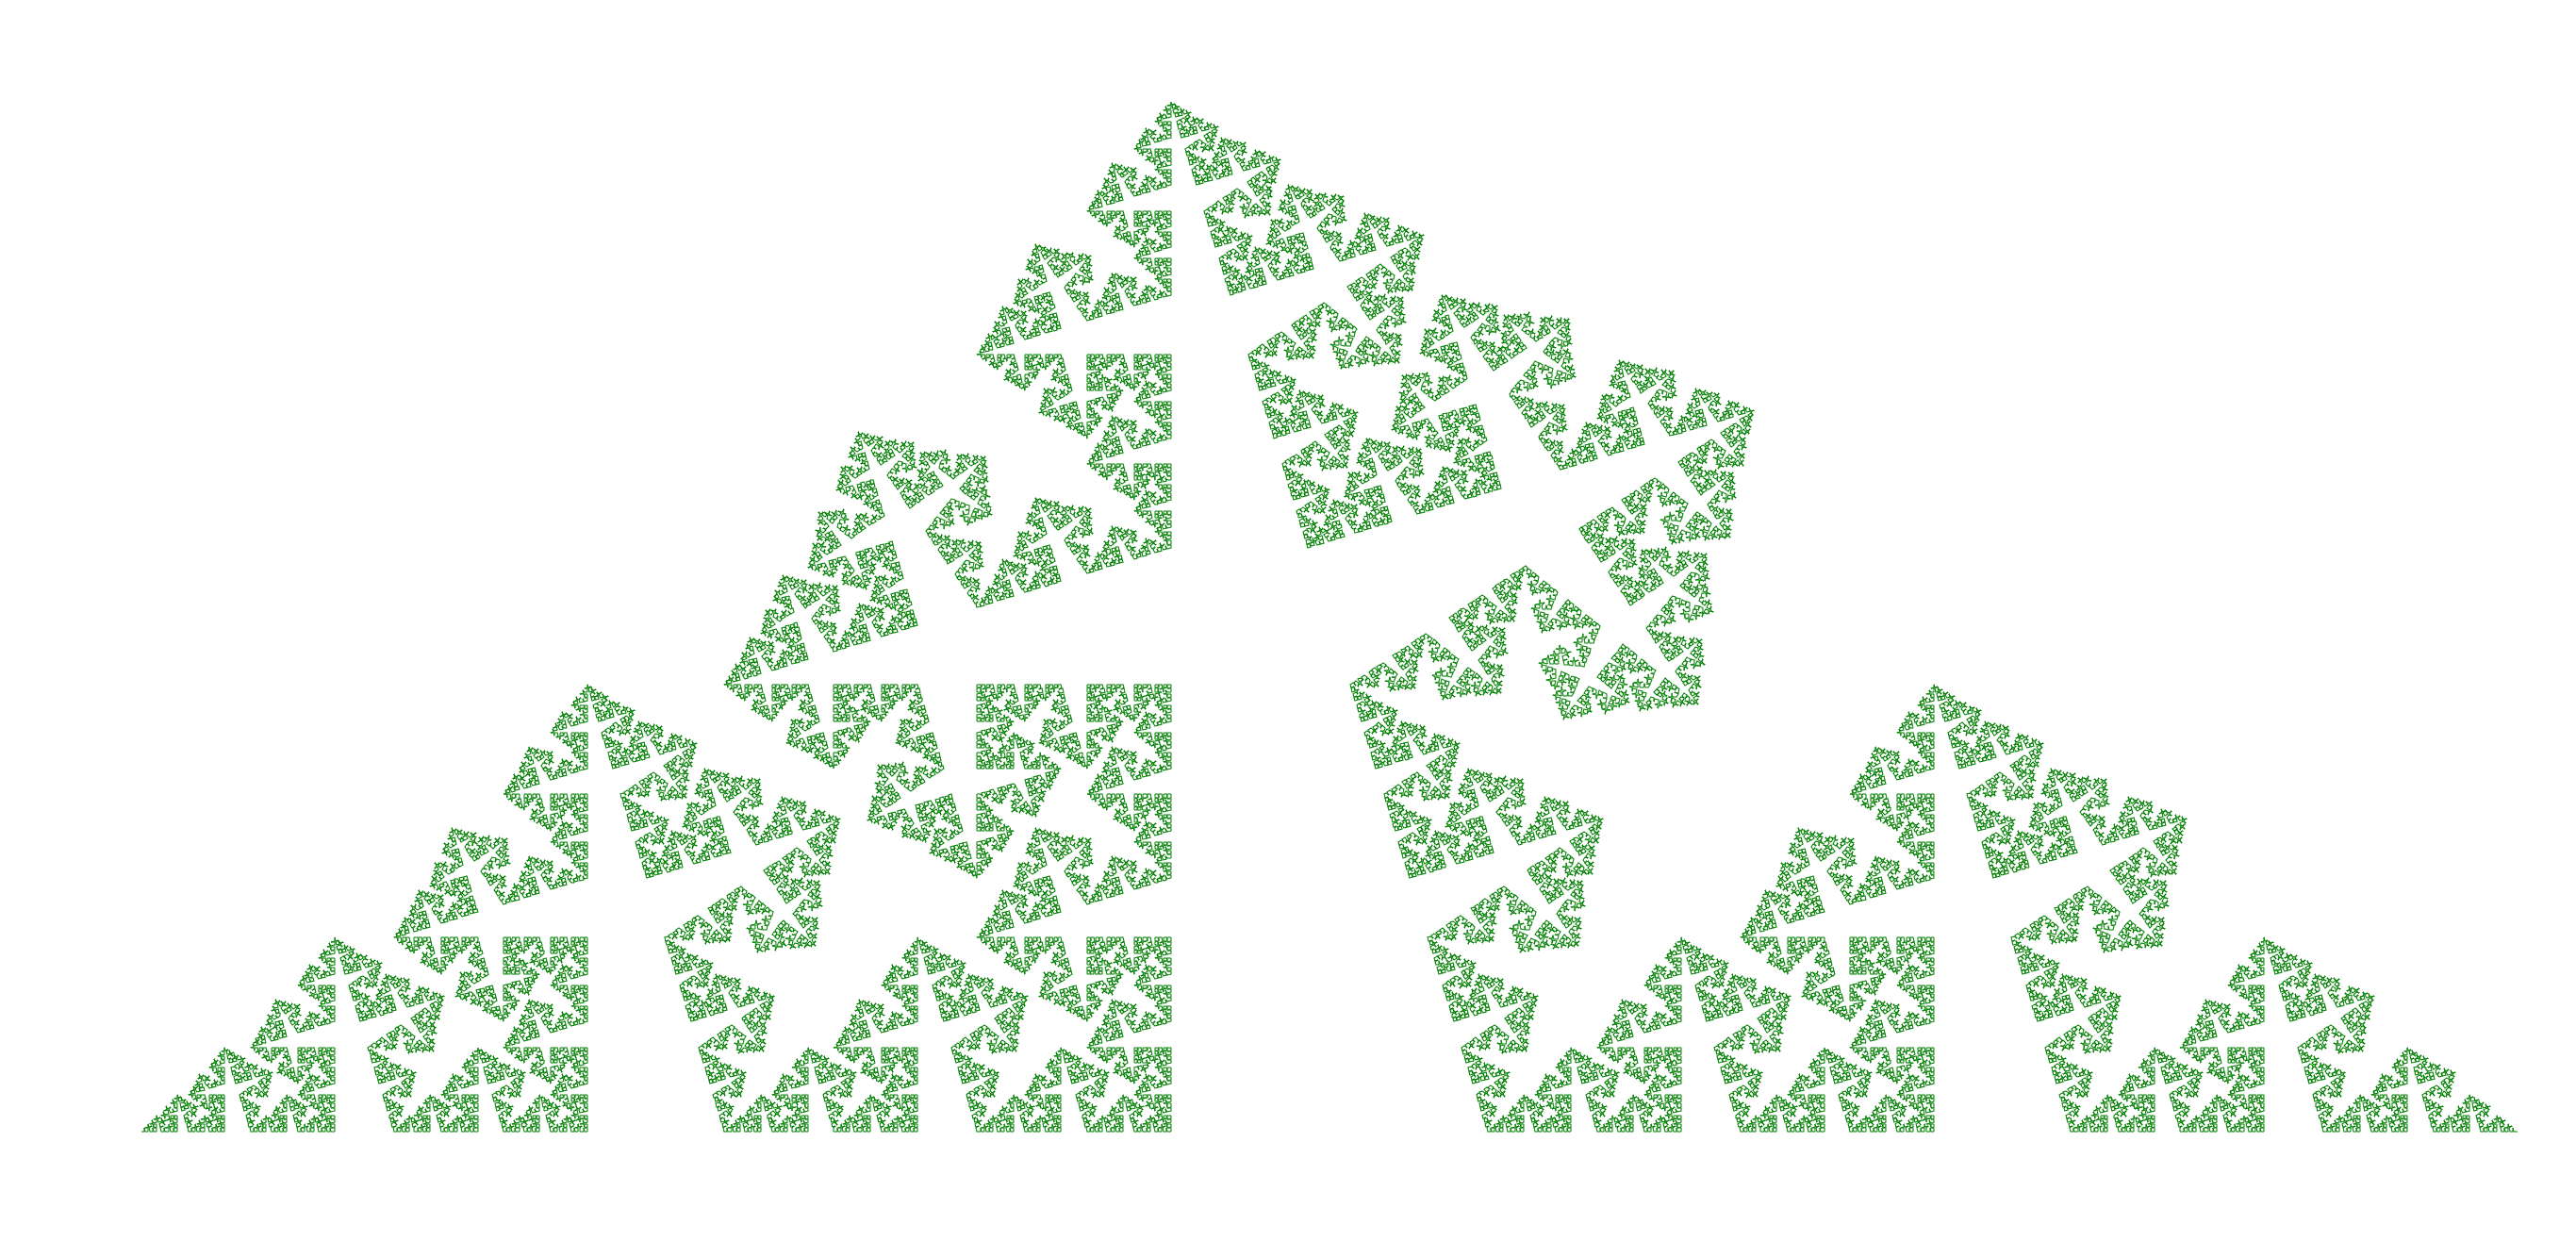
\includegraphics[width=0.49\textwidth]{img/Simple_Variations/koch_variation_01.png}
                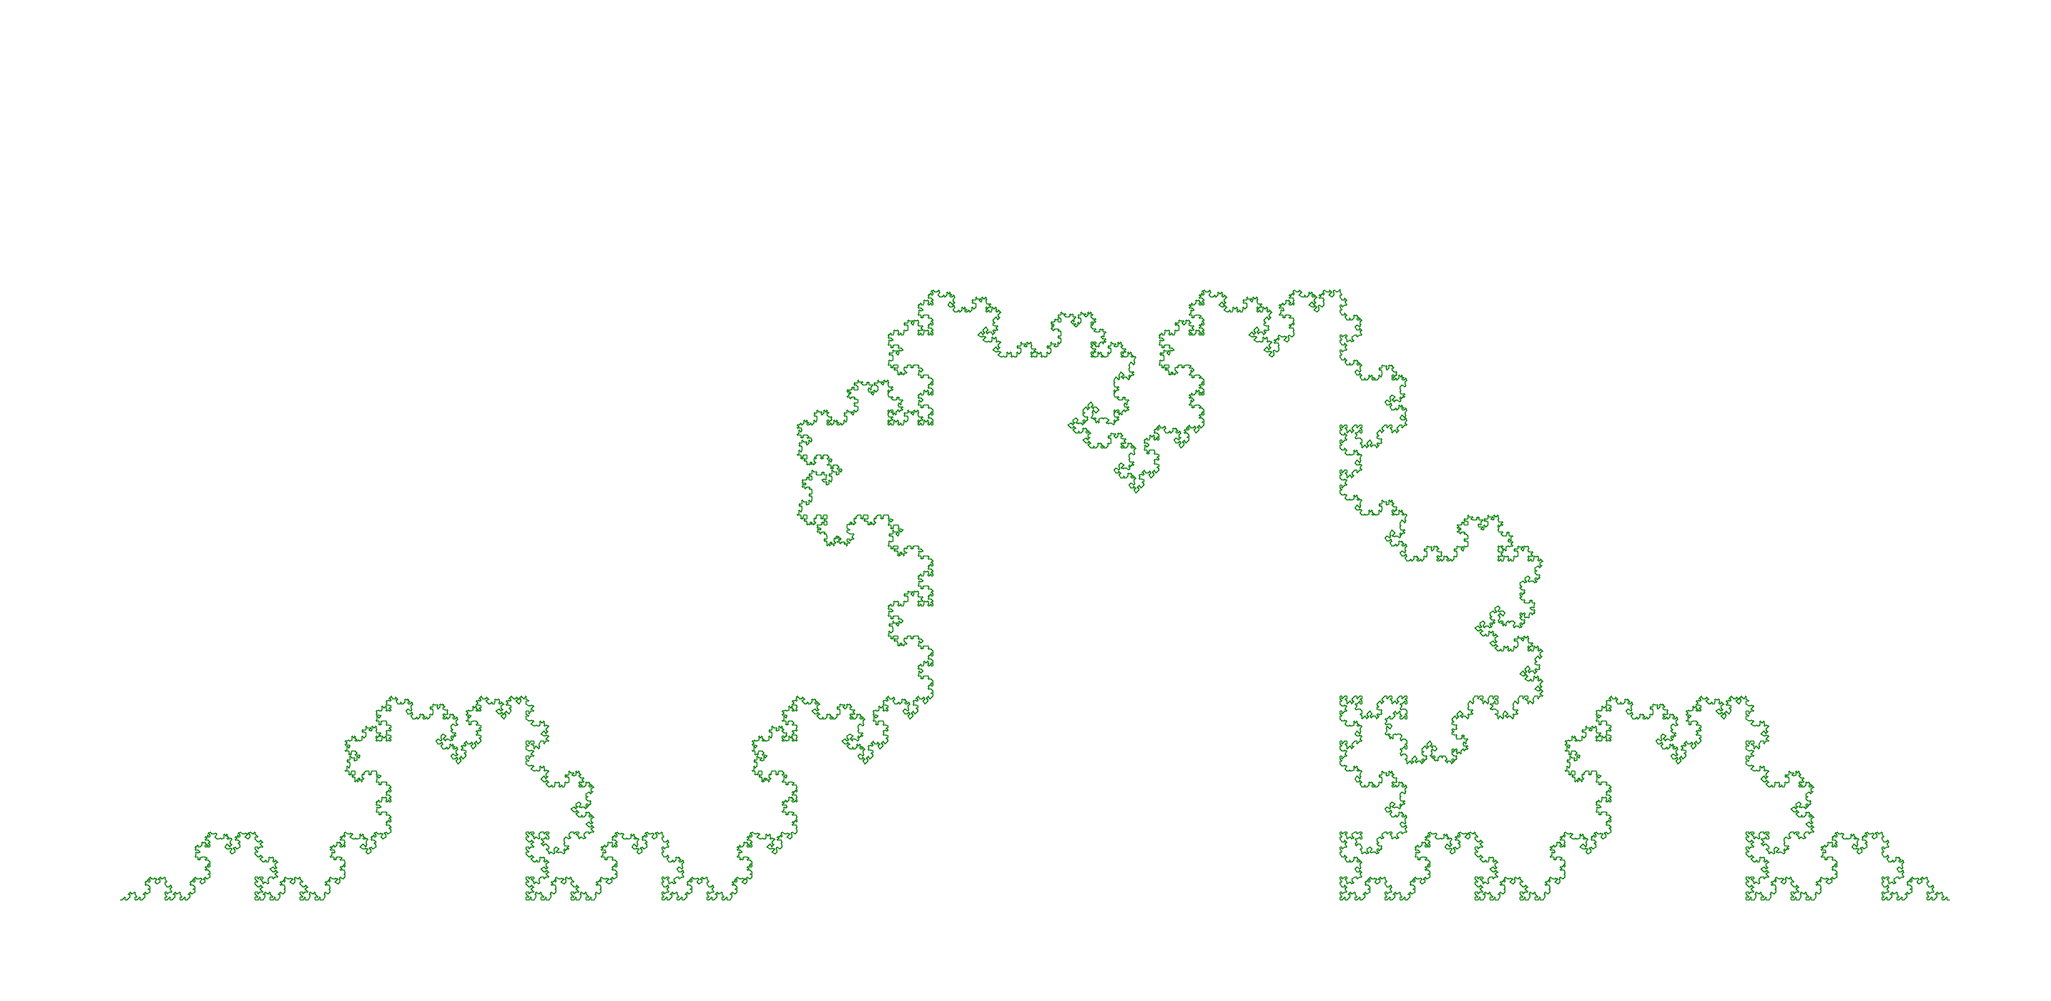
\includegraphics[width=0.49\textwidth]{img/Simple_Variations/koch_variation_02.png}
                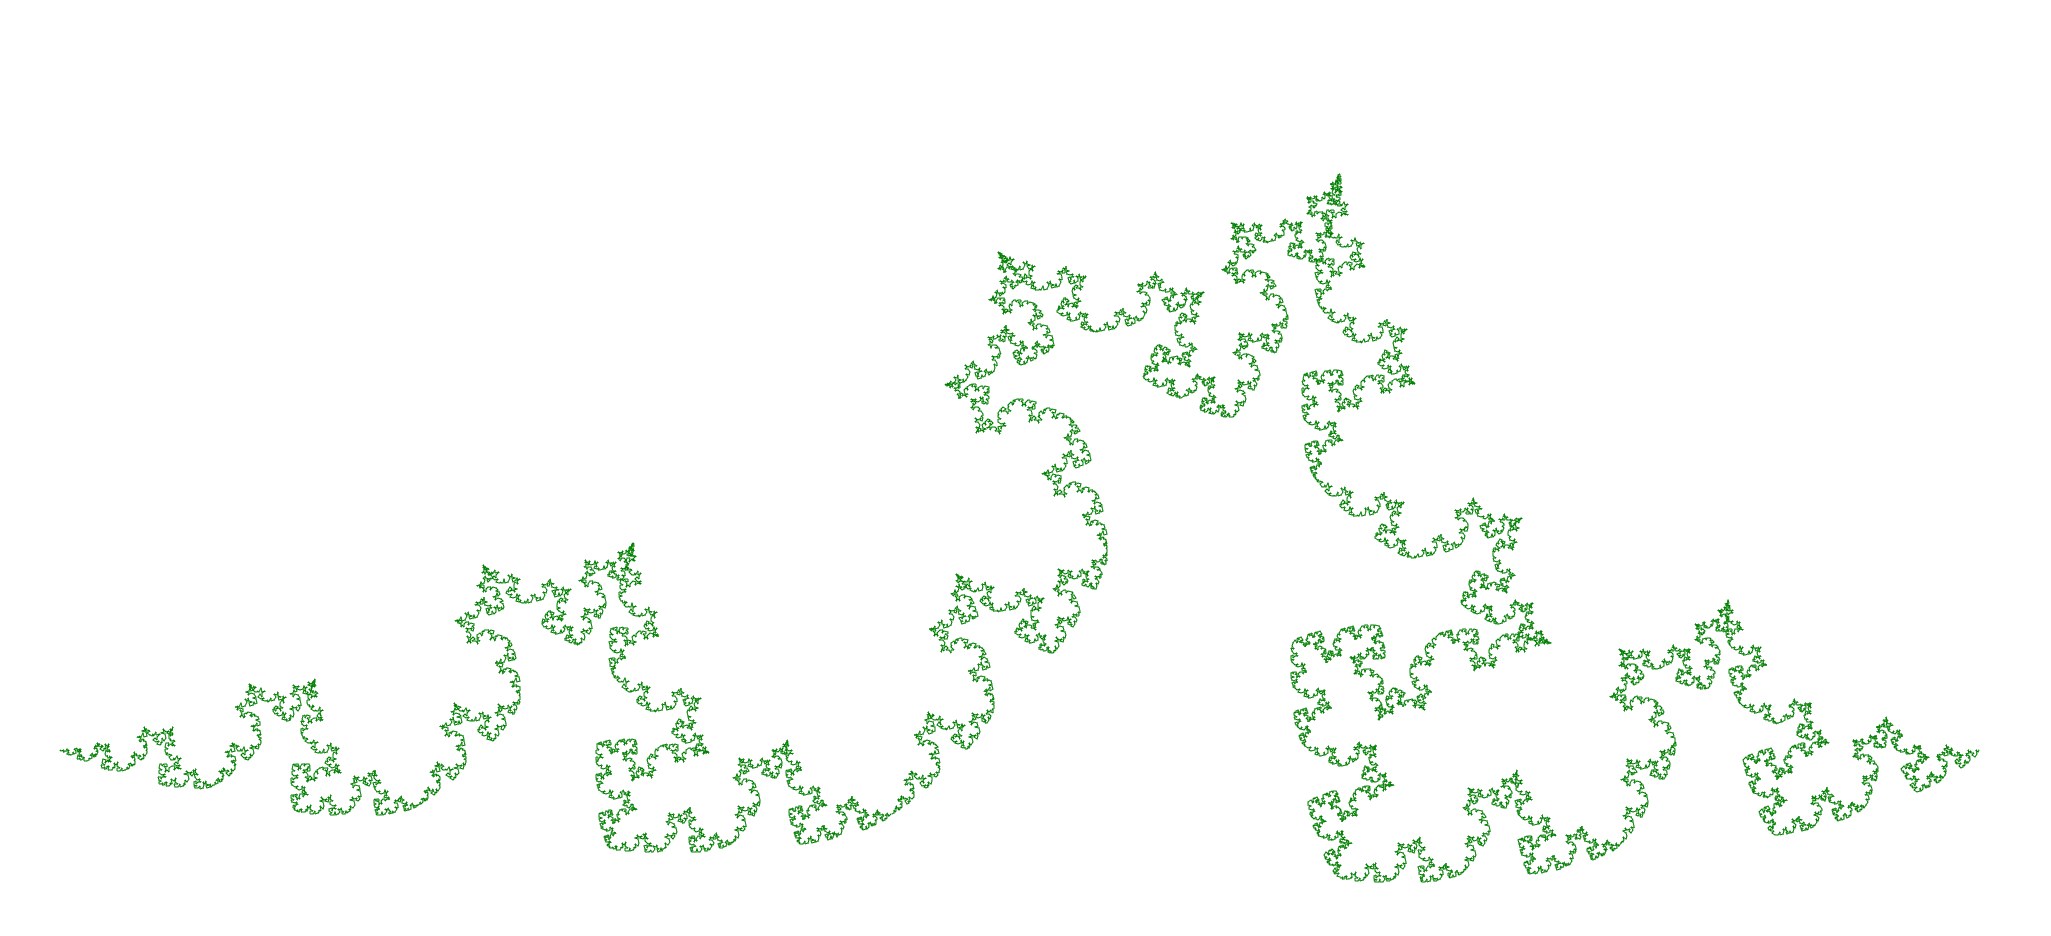
\includegraphics[width=0.49\textwidth]{img/Simple_Variations/koch_variation_03.png}
                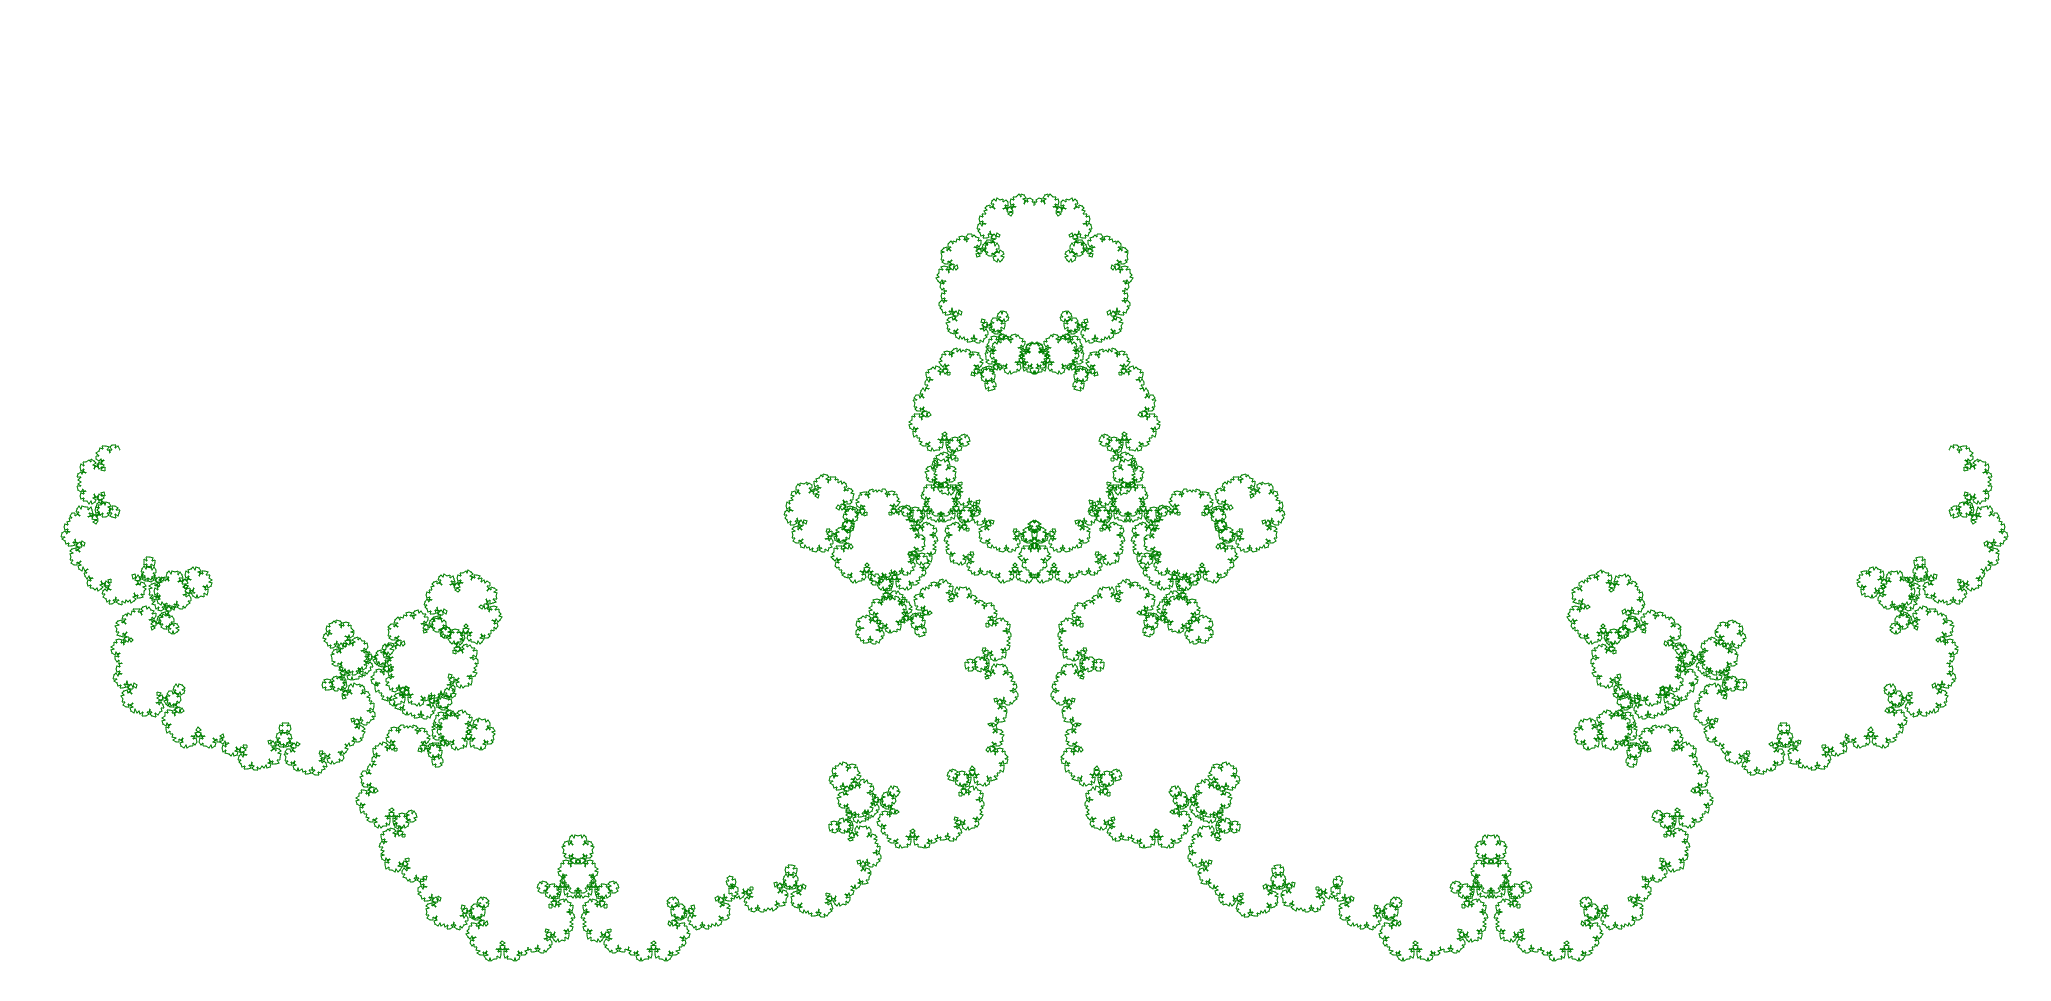
\includegraphics[width=0.49\textwidth]{img/Simple_Variations/koch_variation_04.png}
            \end{figure}

            \FloatBarrier

    
    \section{Simple Techniques}
    \subsection{Simple Spirals}
        Spirals can be created by a simple pattern (Fig. \ref{spiral_setup_01}).
        First a identity segment is drawn then, a single segment recurses further.
        We can call the segment that recurses further, \emph{the recursive segment}.
        The type of the spiral depends on the placement of the recursive segment (green in this case).

        \begin{figure}[ht]
            \caption{\label{spiral_setup_01} Setup of a spiral.}
            \centering
            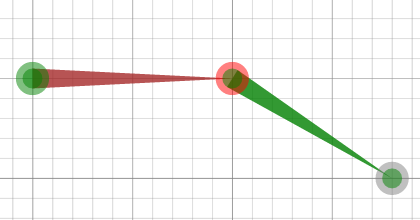
\includegraphics[width=0.4\textwidth]{img/Simple_Techniques/Spirals/spiral_setup_01.png}
        \end{figure}

        \begin{figure}[ht]
            \caption{\label{spiral_simple_01} Simple spirals.}
            \centering
            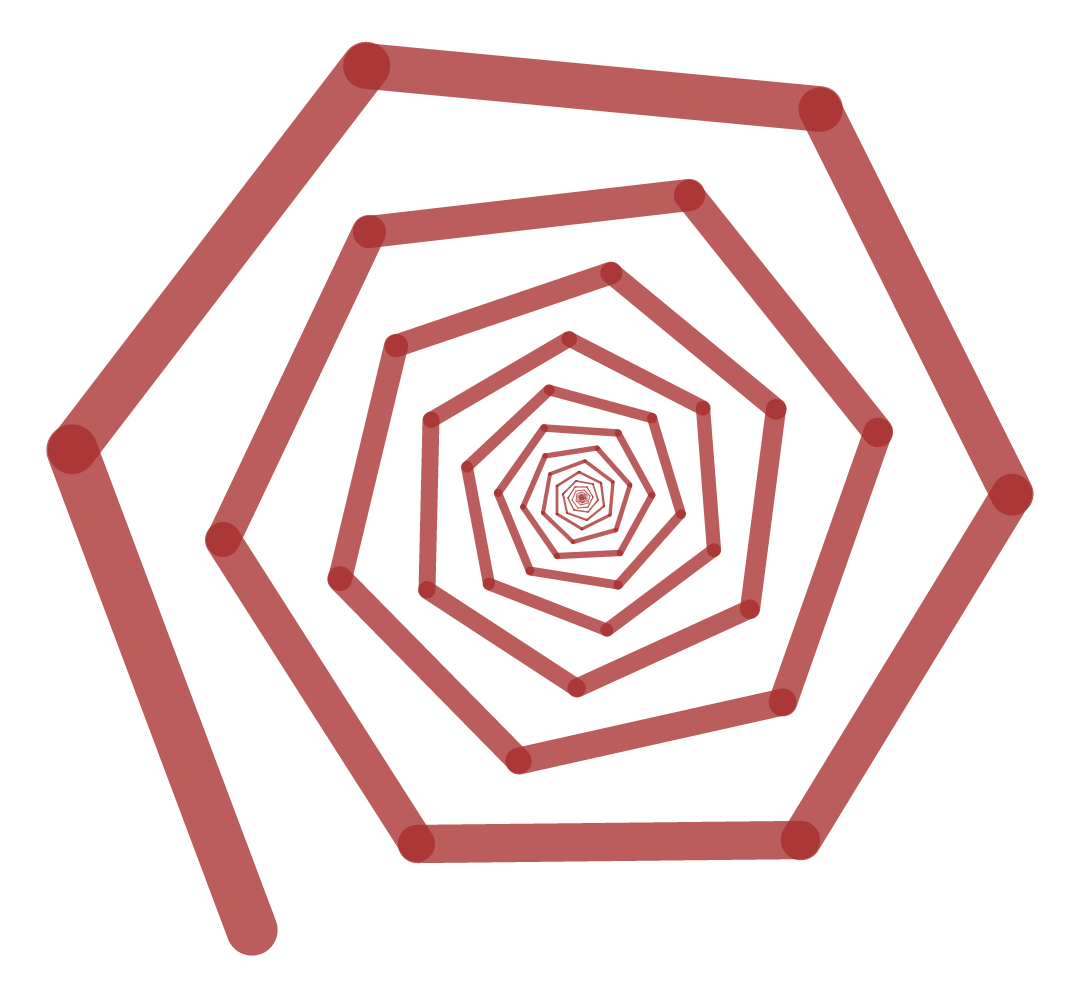
\includegraphics[width=0.24\textwidth]{img/Simple_Techniques/Spirals/spiral_simple_01.png}
            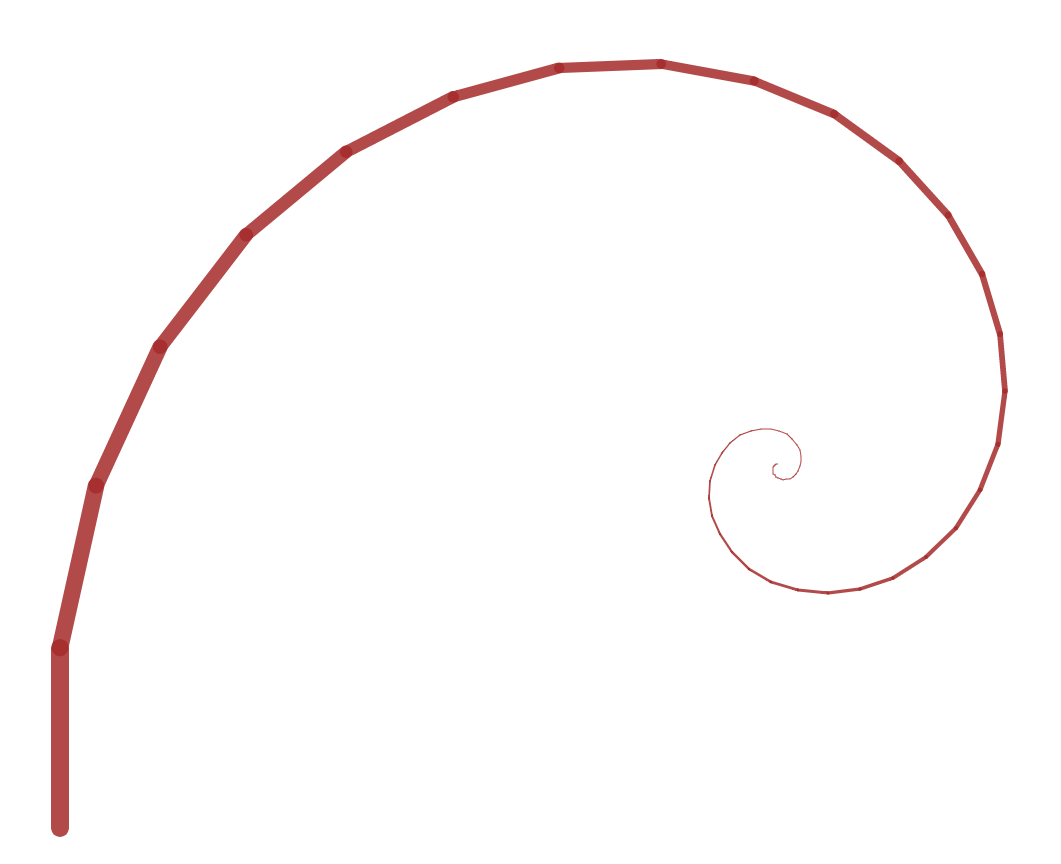
\includegraphics[width=0.24\textwidth]{img/Simple_Techniques/Spirals/spiral_simple_02.png}
            % 
\includegraphics[width=0.24\textwidth]{img/Simple_Techniques/Spirals/spiral_simple_03.png}
            
\includegraphics[width=0.24\textwidth]{img/Simple_Techniques/Spirals/spiral_simple_04.png}
            
\includegraphics[width=0.24\textwidth]{img/Simple_Techniques/Spirals/spiral_simple_05.png}
        \end{figure}


        \FloatBarrier

        \subsubsection{Types of simple spirals}

            The most straightforward way to classify spirals is by the length of their recursive segment.
            Therefore, there are 3 type of spirals.
            The ones which were discussed earlier are the most common type --- \emph{convergent spiral}.
            Convergent spiral are spirals in which the length of the recursive segment is smaller than the length of the identity segment.
            Because of the aforementioned condition, convergent spirals always converge.

            \begin{figure}[ht]
                \centering
                \caption{\label{spiral_diver_01} An example of an divergent and a stationary spiral.}
                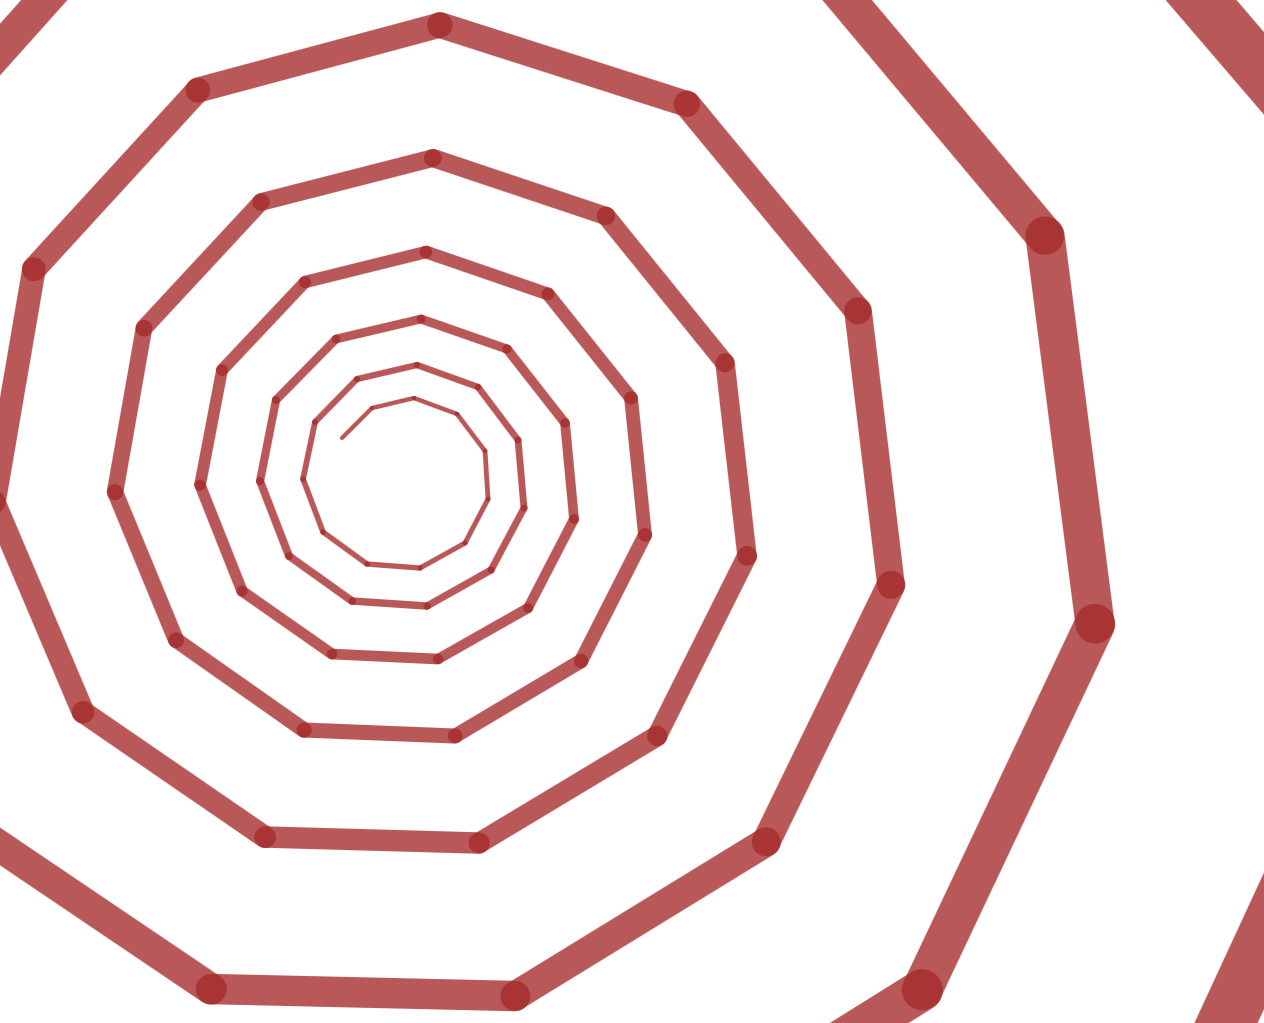
\includegraphics[height=0.2\textwidth]{img/Simple_Techniques/Spirals/spiral_diver_01.png}
                
\includegraphics[height=0.2\textwidth]{img/Simple_Techniques/Spirals/spiral_diver_02.png}
            \end{figure}

            \FloatBarrier


            Besides this, there are of course two other types.
            There are divergent and stationary spirals.
            Usually divergent and stationary spirals are not as interesting as convergent ones, yet, they still can create beautiful figures, as shown in Figure~\ref{spiral_diver_01}.

            As a side note, the best method to create stationary spirals is by using the polar coordinates grid like in Figure~\ref{spiral_diver_setup_01}.
            In this way the length of the segments remain the same and the user has to change only the angle, which is trivial.

            \begin{figure}[ht]
                \centering
                \caption{\label{spiral_diver_setup_01} The setup of a stationary spiral.}
                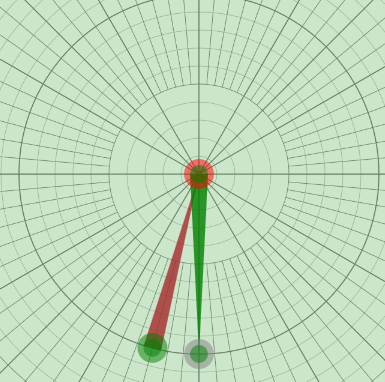
\includegraphics[height=0.3\textwidth]{img/Simple_Techniques/Spirals/spiral_diver_setup_01.png}
            \end{figure}

            \FloatBarrier

        \subsubsection{More interesting spirals}

            An interesting technique is to use two transformations in order to create a single spiral.
            The main one will go in the direction of the rotation of the spiral, as usual, but the second one will go in the opposed direction.
            In this way a zig-zag pattern can be observed.

            \begin{figure}[ht]
                \caption{\label{spiral_simple_02} A more interesting spiral setup.}
                \centering
                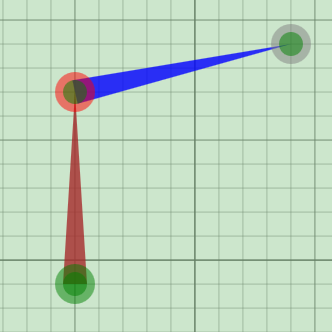
\includegraphics[height=0.3\textwidth]{img/Simple_Techniques/Spirals/spiral_set_02_01.png}
                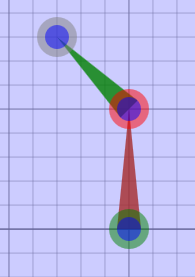
\includegraphics[height=0.3\textwidth]{img/Simple_Techniques/Spirals/spiral_set_02_02.png}
            \end{figure}

            \FloatBarrier

            As it can be observed, the green transformation has a quite long recursion segment.
            This will compensate for the fact that the blue transformation goes in the opposing direction.
            Figure~\ref{spiral_simple_03} shows how such spirals can look.
            One of the figures doesn't even look like a spiral (more like a zig-zagging straight path) but keeping the convention, it will be named like one.

            \begin{figure}[ht]
                \caption{\label{spiral_simple_03} More interesting spirals.}
                \centering
                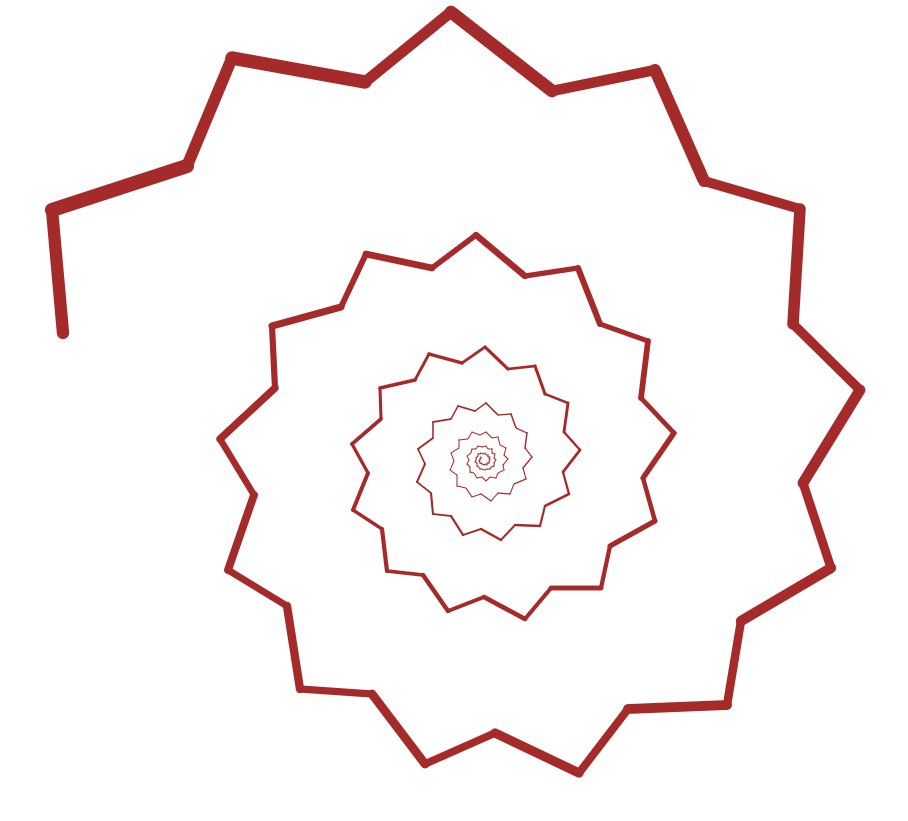
\includegraphics[height=0.2\textwidth]{img/Simple_Techniques/Spirals/spiral_04.png}
                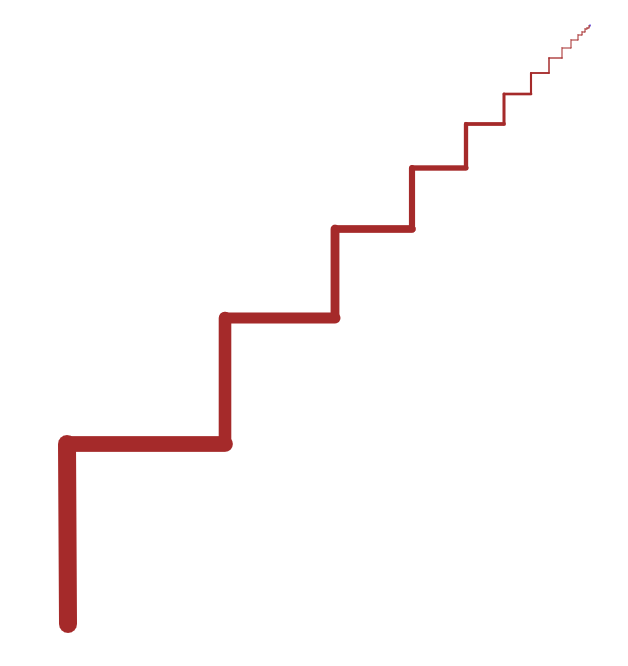
\includegraphics[height=0.2\textwidth]{img/Simple_Techniques/Spirals/spiral_05.png}
                
\includegraphics[height=0.2\textwidth]{img/Simple_Techniques/Spirals/spiral_06.png}
                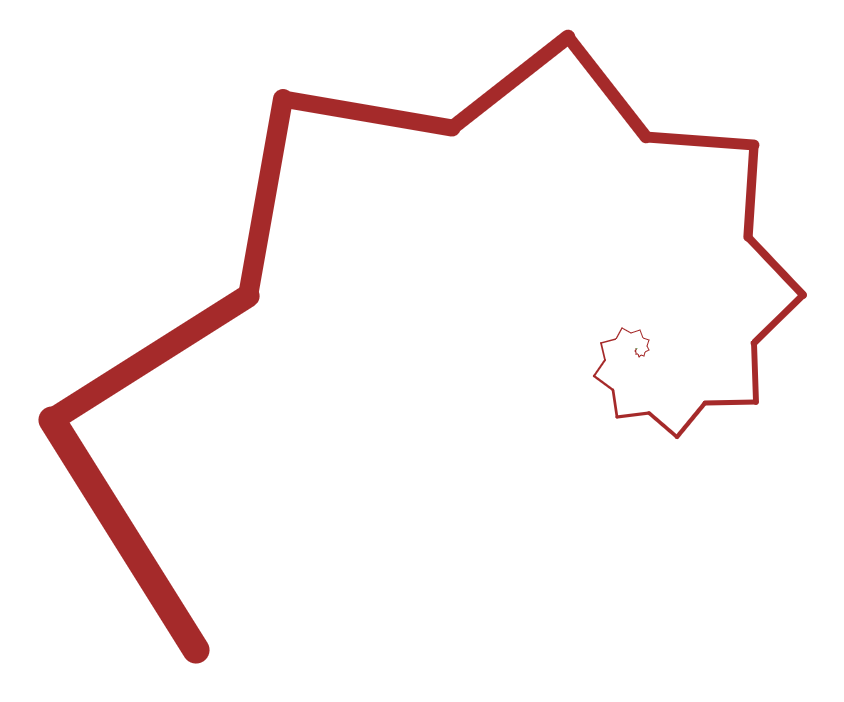
\includegraphics[height=0.2\textwidth]{img/Simple_Techniques/Spirals/spiral_07.png}
            \end{figure}

            \FloatBarrier

    \subsection{Simple Trees}

        By \emph{Tree} I mean not only transformations that resemble trees but also any figure in which a tree-like structure can be distinguished.
        Just as spirals trees can be classified in convergent, divergent and stationary, yet I will only discuss convergent trees since the other two type do not have very interesting features.

        \subsubsection{Trees with two branches}
            Let's begin by creating a figure that resembles the Pythagoras Tree.
            For this particular tree I switched to Polar Coordinates grid so that I could put the branches at exactly 120\textdegree degrees.

            \begin{figure}[ht] 
                \caption{\label{simple_tree_set_01} A geometric tree setup and its corresponding fractal.}
                \centering
                \includegraphics[height=0.3\textwidth]{img/Simple_Techniques/Trees/tree_set_01.png}
                \includegraphics[height=0.4\textwidth]{img/Simple_Techniques/Trees/tree_01.png}
                
            \end{figure}

            Trees look like a natural progression from spirals. 
            Spirals where bound to use just one recursion \emph{branch} whereas trees can use two, or more, as we'll see further.

            Figure~\ref{simple_tree_02} shows some possible types of trees. 

            \begin{figure}[ht]
                \caption{\label{simple_tree_02} Some trees.}
                \centering
                \includegraphics[width=0.27\textwidth]{img/Simple_Techniques/Trees/tree_02.png}
                \includegraphics[width=0.27\textwidth]{img/Simple_Techniques/Trees/tree_03.png}
                \includegraphics[width=0.27\textwidth]{img/Simple_Techniques/Trees/tree_04.png}
                \includegraphics[width=0.27\textwidth]{img/Simple_Techniques/Trees/tree_05.png}
                \includegraphics[width=0.27\textwidth]{img/Simple_Techniques/Trees/tree_06.png}
                \includegraphics[width=0.27\textwidth]{img/Simple_Techniques/Trees/tree_07.png}                
            \end{figure}

            \FloatBarrier

            Some of these trees start to degenerate to spirals with an added node. 
            I will come back to these types of spirals later.

        \subsubsection{Trees with multiple branches}

            Figure~\ref{simple_tree_03} shows some examples of trees with multiple branches.
            Usually having many branches results in getting a clustered fractal so choosing a good transformation is very important.
            

            \begin{figure}[ht]
                \caption{\label{simple_tree_03} Trees with several branches.}
                \centering
                \includegraphics[width=0.32\textwidth]{img/Simple_Techniques/Trees/tree_08.png}
                \includegraphics[width=0.32\textwidth]{img/Simple_Techniques/Trees/tree_09.png}
                \includegraphics[width=0.32\textwidth]{img/Simple_Techniques/Trees/tree_10.png}             
            \end{figure}

            \FloatBarrier

        \subsubsection{Trees with multiple transformations}

            A much more interesting progression from simple trees is to use different transformations that call each other, just like in the beginning of the paper.

            \begin{figure}[ht]
                \caption{\label{simple_tree_set_02} Setup of a tree with two transformations.}
                \centering
                \includegraphics[height=0.3\textwidth]{img/Simple_Techniques/Trees/tree_set_02.png}
                \includegraphics[height=0.3\textwidth]{img/Simple_Techniques/Trees/tree_set_03.png}  
                \includegraphics[width=0.6\textwidth]{img/Simple_Techniques/Trees/tree_12.png}          
            \end{figure}

            \FloatBarrier

            The reader should experiment and see whether he or she can find interesting types of trees using just these simple techniques.

    \subsection{Unconnected figures}
        Until now every transformation implied some kind of connection between segments.
        This is not necessary.
        We can easily create transformations without connections.
        Understanding the mathematical reasoning behind these type of transformations is very important.
        
        Let's start with two adjacent segment, which are not connected to the start nor the end point.
        Figure~\ref{simple_un_line_01} shows the setup.
        The progression shows how the lines evolve.

        \begin{figure}[H]
            \caption{\label{simple_un_line_01} Two segments.}
            \centering
            \includegraphics[width=1.0\textwidth]{img/Simple_Techniques/Unconnect/simple_un_lines_01.png}         
        \end{figure}

        The reasoning behind these transformations may seem rather obscure so let's go through it step by step.
        We start with a segment with the direction showed by the arrow.
        The transformation is superimposed (Fig.~\ref{simple_un_line_exp_01}).

        \begin{figure}[H]
            \caption{\label{simple_un_line_exp_01} The transformation step by step.}
            \centering
            \subcaptionbox{}[0.3\textwidth]
                {\includegraphics[height=0.3\textwidth]{img/Simple_Techniques/Unconnect/simple_line_exp_01.png}}
            ~
            \subcaptionbox{}[0.3\textwidth]
                {\includegraphics[height=0.3\textwidth]{img/Simple_Techniques/Unconnect/simple_line_exp_02.png}}
        \end{figure}
        \FloatBarrier

        Now, it should be clear how the mechanics of the transformation works.
        The arrows are very important, changing the direction of the arrow, usually, completely changes the visual aspect of the figure.

        A major problem with unconnected transformations is that they can diverge to 
            figures that are hard to observe since they are composed from very small parts.
        It is possible to create unconnected transformation with only one recursing segment but the behavior is trivial, 
            so the minimum segments for constructing an unconnected transformation (and actually any type of transformation) is two.

        When it comes to unconnected transformations the result is usually quite unexpected.
        It is hard to guess the final figure just by looking at the transformation.
        Figure~\ref{simple_un_triangle_01} shows an example.

        Sometimes, especially when dealing with unconnected transformations it is best to not iterate very deep.
        For example, in fig.~\ref{simple_un_quad_01} the iteration level is just 5.
        Also observe how unexpected the result is comparing to the setup.
        Some special cases of unconnected transformation will be discussed in further chapters.

        \begin{figure}[ht]
            \caption{\label{simple_un_triangle_01} A unconnected transformation with a triangle}
            \centering
            \subcaptionbox{}[0.2\textwidth]
                {\includegraphics[width=0.2\textwidth]{img/Simple_Techniques/Unconnect/simple_un_setup_triangle_01.png}}
            \subcaptionbox{}[0.7\textwidth]
                {\includegraphics[width=0.6\textwidth]{img/Simple_Techniques/Unconnect/simple_un_triangle_01.png}}
        \end{figure}

        \FloatBarrier

        \begin{figure}[ht]
            \caption{\label{simple_un_quad_01} A unconnected transformation with a figure.}
            \centering
            \subcaptionbox{}[0.2\textwidth]
                {\includegraphics[width=0.2\textwidth]{img/Simple_Techniques/Unconnect/simple_un_setup_quad_01.png}}
            \subcaptionbox{}[0.7\textwidth]
                {\includegraphics[width=0.6\textwidth]{img/Simple_Techniques/Unconnect/simple_un_quad_01.png}}
        \end{figure}

        \FloatBarrier

    \subsection{Singleton Pattern}

        Suppose we have the following setup (fig.~\ref{simple_singleton_01}).
        This is the dragon curve with a square inside.
        Looking at the fractal after some iterations (fig.~\ref{simple_singleton_02}) it is clear that this is not a very aesthetically pleasing fractal.
        It would be much better if only the squares from the last iterations were seen.

        \begin{figure}[ht]
            \caption{An example.}
            \centering
            \subcaptionbox{\label{simple_singleton_01} The setup.}[0.3\textwidth]
                {\includegraphics[width=0.3\textwidth]{img/Simple_Techniques/Singleton/simple_singleton_01.png}}
            \subcaptionbox{\label{simple_singleton_02} After some iterations}[0.65\textwidth]
                {\includegraphics[width=0.6\textwidth]{img/Simple_Techniques/Singleton/simple_singleton_02.png}}
        \end{figure}

        The Singleton pattern solves this problem.
        First we need to create a new type of transformation (fig.~\ref{simple_single_03}).
        It may be strange that the transformation for a singleton pattern doesn't require any segments,
            but the value of this pattern will itself.

        \begin{figure}[ht]
            \caption{\label{simple_single_03} The singleton transformation.}
            \centering
            \includegraphics[width=0.3\textwidth]{img/Simple_Techniques/Singleton/simple_single_setup_02.png}
        \end{figure}

        Let's try to change the dragon curve example on more time, this time using the blue layer (fig.~\ref{simple_singleton_03}).
        In this case the final result looks like this (fig.~\ref{simple_singleton_04}).
        The logic behind this is quite clear, on every iteration a new pair of squares forms but the last one iterates into the singleton transformation and disappears.

        \begin{figure}[ht]
            \caption{Using the singleton pattern.}
            \centering
            \subcaptionbox{\label{simple_singleton_03} The setup.}[0.3\textwidth]
                {\includegraphics[width=0.3\textwidth]{img/Simple_Techniques/Singleton/simple_single_setup_03.png}}
            \subcaptionbox{\label{simple_singleton_04} After some iterations}[0.65\textwidth]
                {\includegraphics[width=0.6\textwidth]{img/Simple_Techniques/Singleton/simple_single_02.png}}
        \end{figure}

        \FloatBarrier

        Instead of just square we can use any type of figure (fig.\ref{simple_single_05}).

        \begin{figure}[ht]
            \caption{\label{simple_single_05} Some examples.}
            \centering
            \includegraphics[width=0.4\textwidth]{img/Simple_Techniques/Singleton/simple_single_03.png}
            \includegraphics[width=0.4\textwidth]{img/Simple_Techniques/Singleton/simple_single_04.png}
        \end{figure}

        \FloatBarrier

        In the previous example only the dragon curve was used.
        This was due to the fact that it was easier to explain using it, nevertheless singleton pattern can be applied in a big variety of cases.
        

    \subsection{Decorator Pattern}

        The definition of the decorator pattern is more abstract than the definition of the previous patterns.
        The idea is to divide segments in two parts. 
        One that is responsible for the recursion mechanics and the other one responsible for the visual setup.

        Let's review the dragon curve example from the previous chapter but make some changes.
        We will use a singleton transformation and the setup will be the same (fig.~\ref{simple_singleton_03}).
        This time, however, I will use a interesting property of the software.
        Inside the color-choosing window there is a gray square with an X inside.
        Pressing that square will make the segments of this transformation completely transparent.
        In this way, the green segments will not be seen, only the blue squares.

        \begin{figure}[ht]
            \centering
            \subcaptionbox{}[0.3\textwidth]
                {\includegraphics[width=0.3\textwidth]{img/Simple_Techniques/Decorator/simple_deco_01.png}}
            ~
            \subcaptionbox{}[0.6\textwidth]
                {\includegraphics[width=0.6\textwidth]{img/Simple_Techniques/Decorator/simple_deco_02.png}}
        \end{figure}

    \subsection{Case Studies}
        
        \subsubsection{Two Rays}

            The title might be misleading since we are not actually dealing with mathematical rays.
            Figure~\ref{ray_01} shows the setup and the figure that it creates.

            \begin{figure}[H]
                \centering
                \caption{\label{ray_01} Two Rays}
                \subcaptionbox{The setup}[0.18\textwidth]
                    {\includegraphics[width=0.18\textwidth]{img/Simple_Techniques/Cases/rays/ray_set_01.png}}
                ~
                \subcaptionbox{The fractal.}[0.78\textwidth]
                    {\includegraphics[width=0.78\textwidth]{img/Simple_Techniques/Cases/rays/ray_01.png}}
            \end{figure}

            It's probably clear why the name \quotes{Rays} was chosen.

            Since the segments are not connected to each other, the final fractal is unconnected.
            This doesn't mean that the segments cannot overlap, this is actually a very common feature of unconnected fractals.

            If we change the setup we can get an interesting fractal (fig.\ref{ray_02}).
            The fractal is similar to the Dragon Curve.
            Even though the segments are unconnected, this fractals shows a interesting type of connection.


            \begin{figure}[H]
                \centering
                \caption{\label{ray_02} The Ray Dragon.}
                \subcaptionbox{The setup}[0.3\textwidth]
                    {\includegraphics[width=0.3\textwidth]{img/Simple_Techniques/Cases/rays/ray_set_02.png}}
                ~
                \subcaptionbox{The fractal.}[0.65\textwidth]
                    {\includegraphics[width=0.65\textwidth]{img/Simple_Techniques/Cases/rays/ray_02.png}}

                \subcaptionbox{First iterations.}[1\textwidth]
                    {\includegraphics[width=1\textwidth]{img/Simple_Techniques/Cases/rays/ray_03.png}}
            \end{figure}

            Moving the segments around we can get other types of strange fractals.
            We can try to invert the arrows, that is, change their direction.
            There are 4 combination in total, below are all the combination applied to the same set of points.

            \begin{figure}[H]
                \centering
                \caption{\label{ray_04} Combination 1.}
                \subcaptionbox{The setup}[0.2\textwidth]
                    {\includegraphics[width=0.2\textwidth]{img/Simple_Techniques/Cases/rays/ray_set_04.png}}
                ~
                \subcaptionbox{The fractal.}[0.78\textwidth]
                    {\includegraphics[width=0.78\textwidth]{img/Simple_Techniques/Cases/rays/ray_04.png}}
            \end{figure}

            \begin{figure}[H]
                \centering
                \caption{\label{ray_06} Combination 2.}
                \subcaptionbox{The setup}[0.2\textwidth]
                    {\includegraphics[width=0.2\textwidth]{img/Simple_Techniques/Cases/rays/ray_set_06.png}}
                ~
                \subcaptionbox{The fractal.}[0.78\textwidth]
                    {\includegraphics[width=0.78\textwidth]{img/Simple_Techniques/Cases/rays/ray_06.png}}
            \end{figure}

            \begin{figure}[H]
                \centering
                \caption{\label{ray_05} Combination 3.}
                \subcaptionbox{The setup}[0.2\textwidth]
                    {\includegraphics[width=0.2\textwidth]{img/Simple_Techniques/Cases/rays/ray_set_05.png}}
                ~
                \subcaptionbox{The fractal.}[0.78\textwidth]
                    {\includegraphics[width=0.78\textwidth]{img/Simple_Techniques/Cases/rays/ray_05.png}}
            \end{figure}

            

            \begin{figure}[H]
                \centering
                \caption{\label{ray_07} Combination 4.}
                \subcaptionbox{The setup}[0.2\textwidth]
                    {\includegraphics[width=0.2\textwidth]{img/Simple_Techniques/Cases/rays/ray_set_07.png}}
                ~
                \subcaptionbox{The fractal.}[0.78\textwidth]
                    {\includegraphics[width=0.78\textwidth]{img/Simple_Techniques/Cases/rays/ray_07.png}}
            \end{figure}


            As we can observe the long segment changes the general aspect of the fractal whilst the smaller ones changes the details of the fractal.

            As a final note, the small segment can be substituted with anything else, for example a tree.

            \begin{figure}[H]
                \centering
                \caption{\label{ray_08} Tree in spiral.}
                \includegraphics[width=0.6\TW]{img/Simple_Techniques/Cases/rays/ray_08.png}
            \end{figure}

    \section{Advanced Techniques}

	\subsection{Step-by-step pattern}

		The Step-by-step pattern was used previously in the book.
		It is very useful to use it for observation purposes, that is, to observe how a fractal evolves over time.
		
	    Suppose that Layer 1 has a simple transformation, for example the Koch Snowflake.
	    Then suppose that Layer 2 has the following transformation (fig.\ref{step_01}).

	    \begin{figure}[H]
	    	\centering
	    	\caption{\label{step_01} Step-by-step pattern.}
	    	\subcaptionbox{Koch Snowflake.}[0.3\TW]
                {\includegraphics[height=0.3\TW]{img/Advanced_Techniques/Step/step_set_02.png}}
            ~
            \subcaptionbox{Step-by-step pattern.}[0.3\TW]
                {\includegraphics[height=0.3\TW]{img/Advanced_Techniques/Step/step_set_01.png}}
	    \end{figure}

	    \begin{figure}[H]
	    	\includegraphics[width=0.9\TW]{img/Advanced_Techniques/Step/step_01.png}
	    \end{figure}

	    Layer 2 works by creating a desired iteration and then calling himself a little further.
	    In this way the development of the fractal becomes very clear.
	    Of course it is not necessary that the segments in the Step-by-step transformation should be parallel to each other.
	    We can choose a circular configuration.
	    The blue color can be removed by pressing the X in color-choosing dialog.

	    \begin{figure}[H]
	    	\centering
	    	\caption{\label{step_03} Step-by-step pattern.}
	    	\subcaptionbox{The setup.}[0.25\TW]
                {\includegraphics[width=0.25\TW]{img/Advanced_Techniques/Step/step_set_03.png}}
            ~
            \subcaptionbox{The fractal.}[0.5\TW]
                {\includegraphics[width=0.5\TW]{img/Advanced_Techniques/Step/step_03.png}}
	    \end{figure}

	\subsection{Color Mixing}

		This is more of a trick than a relevant mathematical concept.
		While a complex figure is being drawn, the user can choose a different color for the segments.
		Figure~\ref{mix_01} shows this technique applied to the dragon curve.

		\begin{figure}[H]
			\centering
			\caption{\label{mix_01} Colored Dragon}
	    	\includegraphics[width=0.8\TW]{img/Advanced_Techniques/Mixing/mix_01.png}
	    \end{figure}

    \section{Randomness}

	Until now, every transformation had a deterministic figure.
	Usually, for fractals, this is a important behavior but sometimes some randomness would be useful.
	For example suppose we want to simulate some trees.
	Every tree created should have a different type of transformation.
	Even if we use different starting segments, the trees will have similar behavior.
	What to do then in order to create a forest of trees.
	Randomness is the answer.

	In his book ``A new Kind of Science'', Stephen Wolfram discusses about the fact that randomness can arise from within a simple system without interaction from other systems (external factors).
	For exemplifying this, he uses different types of finite automata.

	In finite automata, the further development of a cell can be influenced by it's surroundings.
	His finite automata are placed in discrete space and can easily have access to their surroundings.
	I found it harder to reproduce this behavior for systems which are placed in continuous space.

	For example a segment could recurse further or stop depending on whether it crosses another segment.
	Or the type of the segment could be influenced by the number of segments in a certain proximity.

	The implementation of these functionalities into the software would take away its minimalism.
	That is the reason I chose (for now) some other methods for creating randomness.
	Unfortunately these methods rely on external factors.

	\subsection{Node position variation}

		Suppose we have setup of a simple tree (fig.~\ref{ran_tree_01}).
		It will create a very basic fractal.
		In order to add some randomness the following should be done by the user.
		Press \emph{CTRL} key while dragging the node.
		A blue disc appears around the node (fig.~\ref{ran_tree_02}).
		This blue disc represents the area in which the node can be placed.
		To delete the randomness disc press the \emph{CTRL} key and the middle mouse button.

		One can observe that the creating, deletion buttons retain their meaning,
			only the \emph{CTRL} key is added.

		\begin{figure}[H]
			\centering
			\subcaptionbox{\label{ran_tree_01} A simple tree.}[0.4\textwidth]
				{\includegraphics[height=0.3\textwidth]{img/Randomness/Node/ran_tree_01.png}}
			~
			\subcaptionbox{\label{ran_tree_02} A tree with added randomness.}[0.4\textwidth]
				{\includegraphics[height=0.3\textwidth]{img/Randomness/Node/ran_tree_02.png}}
		\end{figure}

		Figure~\ref{ran_tree_03} shows some possible trees.
		All the trees were created using the same starting segment.

		\begin{figure}[H]
			\centering
			\caption{\label{ran_tree_03} Some random trees.}
			\includegraphics[width=0.9\TW]{img/Randomness/Node/ran_tree_03.png}
		\end{figure}

		The start point and the end point cannot have a random position.
		No node in the base layer can have a random position.

		Let's look at some useful application.

		\subsubsection{Random Paths}

			The setup of a very interesting example can be observed in figure~\ref{ran_path_set_01}.
			Figure~\ref{ran_path_01} shows some of the figures, superimposed.

			\begin{figure}[H]
				\centering
				\caption{Random path.}
				\subcaptionbox{\label{ran_path_set_01} The setup.}[0.3\textwidth]
					{\includegraphics[width=0.29\TW]{img/Randomness/Node/ran_path_01.png}}
				~
				\subcaptionbox{\label{ran_path_01} Some paths.}[0.6\textwidth]
					{\includegraphics[width=0.59\TW]{img/Randomness/Node/ran_path_02.png}}
			\end{figure}

		\subsubsection{Random Spirals}

			Due to the minimalistic nature of spirals, randomness is a very good fit for them.
			I'll start with spirals which do not rotate.

			\begin{figure}[H]
				\centering
				\caption{Straight spirals.}
				\subcaptionbox{\label{ran_spir_set_01} The setup.}[0.3\textwidth]
					{\includegraphics[width=0.29\TW]{img/Randomness/Node/ran_spir_set_01.png}}
				~
				\subcaptionbox{\label{ran_spir_01} Some paths.}[0.6\textwidth]
					{\includegraphics[width=0.59\TW]{img/Randomness/Node/ran_spir_01.png}}
			\end{figure}

			Randomness can be applied to \quotes{real} spirals but that doesn't always result in a beautiful picture.

			\begin{figure}[H]
				\centering
				\caption{\label{ran_spir_02} Some spirals.}
				\includegraphics[width=0.29\TW]{img/Randomness/Node/ran_spir_02.png}
				\includegraphics[width=0.29\TW]{img/Randomness/Node/ran_spir_03.png}
				\includegraphics[width=0.29\TW]{img/Randomness/Node/ran_spir_04.png}
			\end{figure}

    % \section{Mirroring}

	

    % \section{Case Studies}

	\subsection{A different type of spiral}


    
    \section{Used Technologies}
        I started creating this piece of software with the idea that it would be easily used online. That is the reason I used JavaScript, HTML and CSS as the main technologies. Below I will try to explain most of the details and the problem that arised during the development phase.

        \subsection{General HTML layout}

            The main HTML page has several layers stacked one over another. First of all, there are 2 \emph{canvas} elements. One is used for the grid and the other one is used for drawing the recursive image. After this there are several \emph{SVG} elements (I call them \emph{layers} in the code). These layers contain all the draggable elements (the circles, the arrows and the invisible background). Also, for the menu, I used \emph{jQuery UI} framework. That is a simple to use HTML/CSS widget. This is basically all the setup.

        \subsection{The \emph{Canvas} element}
            Wikipedia \cite{wiki_canvas} give a very good and brief description of the canvas. \\
            \emph{The canvas element is part of HTML5 and allows for dynamic, scriptable rendering of 2D shapes and bitmap images. It is a low level, procedural model that updates a bitmap and does not have a built-in scene graph}. \\

            The canvas element has several simple to use functions like \xt{lineTo()}, \xt{moveTo()}, \xt{fill()}, \xt{stroke()}, etc. Canvas is very good and fast at drawing lots of lines and this was exactly what I needed.

            While beginning to work on the project I first implemented the recursive drawing using a SVG element (which I will talk about shortly) but it was to computationally expensive and slow that's why I used canvas.

        \subsection{The \emph{SVG} element}
            The SVG element (Scalable Vector Graphics) is developed since 1999. It uses an XML syntax (just like HTML) to represent vector images. For example in order to represent an circle of radius $r=50$ with the center in coordinates $x=100$ and $y=200$ one should simply write :
            \begin{lstlisting}
            <?xml version="1.0"?>
            <svg viewBox="0 0 120 120" version="1.1"
                xmlns="http://www.w3.org/2000/svg">
                
                <circle cx="100" cy="100" r="50"/>
            </svg>
            \end{lstlisting}
            
            Actually all the text before \xt{<circle />} is just telling what version of SVG standard we are using. Omitting most of those lines would usually not be a problem.

            As it can be deduced SVG is great at, well, displaying vector graphics. Because it is written in XML it has a clear hierarchy of the objects inside it. Besides this it can trigger events that can be used by JavaScript code. This is a reason why I used SVG for drawing the draggable parts. For example in order to test whether the user has clicked inside the arrow (which is basically a triangle) I would had to use some geometric calculations. Using SVG I just used the \xt{click()} event. The same is for the circles.

            It should be noted that SVG is used not just in web browsers. There are some vector graphics editors which use SVG as the primary standard (Inkscape).

        \subsection{Snap SVG} 
            Working with pure JavaScript functions for editing the SVG can be tedious and error prone. That is the reason I used a small framework, Snap.svg. 
            Snap has a lot of functionality, at least more than I needed. 
            It can perform animation, matrix transformation, filtering, etc. But I used just a little part of them. 
            The most useful function was \xt{attr()}. 
            That is a versatile function that can get or set attributes of SVG elements. For example instead of writing:
            \begin{lstlisting}
            cirle.setAttribute('cx', 5);
            cirle.setAttribute('cy', 89);
            cirle.setAttribute('r',  34);
            \end{lstlisting}
                        I could just write

            \begin{lstlisting}
            circle.attr({
                'cx', 5,
                'cy', 89,
                'r',  34
            });
            \end{lstlisting}
            which is easier to write and read. 

            Snap.svg has similar function for creating and deleting elements. These functions where widely used inside the code of the software.

        \subsection{jQuery UI}
            One of the most used JavaScript framework is jQuery. A very good explanation of what jQuery UI is can be found on their site \cite{jquery}. \\
            \emph{jQuery UI is a curated set of user interface interactions, effects, widgets, and themes built on top of the jQuery JavaScript Library.}

            In order to use jQuery UI one should simply add an \xt{div} or \xt{input} element inside the HTML page then invoke some jQuery UI methods in order to apply the needed CSS transformation to that div. For example The code below transforms the div with the id \emph{testing} into a button.
            \begin{lstlisting}
            $('#testing').button();
            \end{lstlisting}

            Of course besides this, jQuery has similar methods for responding to events.

        \subsection{Spectrum.js}

            I needed some way to let the user to choose colors for different layers. 
            Writing such a thing from scratch would not be efficient that's why I used a user-made widget for jQuery UI. 
            The name of that widget is \emph{Spectrum.js}. 
            It provides some simple way of configuration and, generally, didn't require to much insight to use. 

        \subsection{CoffeeScript}

            CoffeeScript is a little language that compiles into JavaScript. 
            That's what their site claims. 
            Their motto is \quotes{It's just JavaScript}. 
            The language does not implement some different concepts or any other things that would be strange for a JS developer. 
            It just writes more beautiful and more readable code than JS. 
            For example instead of writing.
            \begin{lstlisting}
            test = function() {
                // something
            }
            \end{lstlisting}
            in JavaScript, one could write
            \begin{lstlisting}
            test = () ->
                # something
            \end{lstlisting}
            in CoffeeScript.

            Of course this is a simple example but the lack of the \xt{function} keyword was a big motivation for me to switch to CoffeeScript.

            I will note that there are a lot of languages that compile to JavaScript. Another one worth to mention is TypeScript. TypeScript was developed by a Microsoft employee and provides classes and static typing. 


    \section{Implementation details}

    Before starting the work on this project I did a somehow similar piece of software. 
    That project gave me the idea to implement develop the project that I am currently talking about that I now write about.

    I first wanted to draw the recursive line in a SVG element, I also wanted to draw a grid for every layer. 
    The way the layers are structured in the final version was not thought from the start, it was a process of trial and error.

    The main piece of code was written in a handful of days. 
    It was written in pure JavaScript with very poor architecture. 
    It could draw lines but it was clear that the bugs and the general code repartition would not allow space for further improvements. 

    After struggling some time I decided to use a different approach.
    I decided to rewrite all of my code in CoffeeScript. I never used it or anything alike till then. 
    I had the wrong opinion that CoffeeScript would be to high-level and would hard to debug after transforming it to JavaScript. 
    This was not the case.

    CoffeeScript is a very thing layer over JavaScript.
    Most lines in CoffeeScript can be easily converted to JavaScript, without to much hassle.
    I talked about this before.

    After a day or two I, finally, managed to transform all my code to CoffeeJS.
    The didn't mean that my code got better.
    It still lacked modularity and was generally speaking - bad code.

    Using the CoffeeJS \xt{class} construct I managed to implement a better structured OOP architecture.

    \subsection{The Vector class}

        During all the geometry transformations, lots of times, I had to transform cartesian coordinates to polar coordinates and vice-versa.
        I could create two functions that would transform to and from these coordinates systems.
        But it was clear that using such an approach would be tedious.
        This problem arose at my first project (I talked about it earlier).

        I tried to resolve this by implementing a class that could store and return at the same time both types of coordinates.
        The class had 4 properties : \\
        \xt{orthX, orthY, polarRad, polarAng} 

        These were closure \cite{closures} variables so the user could not access them.
        I provided several methods for interaction, like: \\
        \xt{setX(),  getAng(), getY(), setRad()}, etc.


        Inside these functions, beside setting or returning the requested variable I would recalculate the coordinates.
        For example if a user used \xt{setAng()}, I would set the angle to the given value and, after that, would recalculate the cartesian coordinates.
        In this way, every calculation happened without the knowledge of the user.


        The problem with this was that it was still to cumbersome.
        That was when I found out about a very interesting and obscure feature of JavaScript \cite{defineProperty}.

        \subsubsection{Object.defineProperty}

            Basically this function allows to define all kinds of properties for variables. For example:
            \begin{lstlisting}
            Object.defineProperty(this, 'y', {
                get : function() {
                    return orthY;
                },
                set : function(val) {
                    orthY = val;
                    this.recalcPolar();
                }
            });
            \end{lstlisting}

            This piece of code defines a property \xt{y} that would return the private value \xt{orthY} when used, for example:
            \begin{lstlisting}
            var otherVariable = object.y;
            \end{lstlisting}
            will return the private variable \xt{orthY} from inside the closure of \xt{object}.

            This is doesn't look very useful but the \xt{get} function defines a more interesting behavior. When someone assigns a value to property \xt{y} it not only changes the variable \xt{orthY}, it also recalculates the polar coordinates. For example, the user can use \\
            \begin{lstlisting}
            object.y = 5;
            \end{lstlisting}
            instead of
            \begin{lstlisting}
            object.setY(5);
            \end{lstlisting}

            An even more interesting behavior can be observed below
            \begin{lstlisting}
            object.y += 3;
            \end{lstlisting}
            Here we increase the \xt{y} value the recalculate the points. Writing this using simple functions would look like this:
            \begin{lstlisting}
            object.setY( object.getY() + 3 );
            \end{lstlisting}

            Now the real power of \xt{Object.defineProperty()} can be observed.

    \subsection{Basic Geometry and point transformation}

        After the user moves the points on the SVG layers I needed a way to transform that location of the points to a different line. 
        One of the biggest fears that stopped me from starting to work on this project was that I was not sure how to implement the line transformations. 
        After implementing the Vector class I used a very simple technique.
        This technique will be explained below.

        \subsubsection{Simple Transformation}

            Suppose we have this setup:

            \begin{figure}[ht]
                \centering
                \caption{Initial state of the points.}
                \includegraphics[scale=0.6]{img/explain01.png}
            \end{figure}

            \FloatBarrier

            We have several points. 
            The green one represents the start of the segment and the red one the end of the segment.
            I start by translating the points so that the start point coincides with the center of the coordinate system.
            At the same time I find the angle between the segment that links the start and end point and the X-axis.

            \begin{figure}[ht]
                \centering
                \caption{After translation. The angle.}
                \includegraphics[scale=0.6]{img/explain02.png}
            \end{figure}

            \FloatBarrier

            Now I rotate all the points with that angle so that the end point is on the X-axis.
            All the other point follow by.

            \begin{figure}[ht]
                \centering
                \caption{After translation. The angle.}
                \includegraphics[scale=0.6]{img/explain04.png}
            \end{figure}

            \FloatBarrier

            Finally, I scale all the points such that the end point is on (1, 0) on cartesian coordinates.

            \begin{figure}[ht]
                \centering
                \caption{After scaling.}
                \includegraphics[scale=0.6]{img/explain05.png}
            \end{figure}

            \FloatBarrier

            In such a way the vector that connect the start point with the end point is the X-axis unit vector.

            All these transformation occur inside the function \xt{toUnitVectors()}.
            This function is called from the method \xt{getData()} of the \xt{LineLayer} class.
            Basically the user can call the method on a particular SVG layer and the layer will calculate the data and will return it in a compact form.
            Of course the function \xt{getData()} also returns data about the lines between the points but this is trivial task.

            Here is the code
            \begin{lstlisting}
    toUnitVectors: function(points){
        var ret = [];

        // There should exist at least two points
        if (!(points[1] && points[0])) return;

        // Vector from start point to end point
        var dir = new Vector(points[1].x - points[0].x, points[1].y - points[0].y);
        
        for (var i=0; i<points.length; ++i) {
            // vector from start point to point[i]
            var v = new Vector(points[i].x, points[i].y);

            // Translate the point
            v.x -= points[0].x;
            v.y -= points[0].y;

            // Change angle
            v.ang -= dir.ang;

            // Scale distance
            v.rad /= dir.rad;

            ret.push(v);
        }
        return ret;   
    }
            \end{lstlisting}


        \subsubsection{A faster algorithm}

            One might argue that it would be a better idea to implement something that would not require so much computation and storage.
            For example to use simple matrix transformations and to not use a complex data type like Vector but stick to a simple one, an array of two elements for example.
            This behavior will be probably implemented, but there are other, more important problems that need to be solved. 

    \subsection{Recursive drawing}

        Another problem that I had to tackle is choosing an optimal recursive drawing algorithm.
        The core is clear, I iterate through the segment calling the function recursively till I get to deepness 0 when I draw the line.

        If I would use this simple approach the program might resist for simple drawings but it would completely freeze if there a lot of functions.
        And I think when the number of calls gets to 300000, that can be called a lot of functions.
        Besides this, even if the program might succeed in drawing the segments the user will be unable to move anything while the program is drawing.
        That was a major drawback.

        \subsubsection{Asynchronous JavaScript}

            JavaScript is known as a language than can be easily used for asynchronous function callback.
            You give a function, give a number of milliseconds, and after that time passes the functions is executed.
            There are to basic functions that provide this functionality: \xt{setTimeout(func, millis)} and \xt{setInterval(func, millis)}.
            The first one executes the function just one time, the second executes the function indefinitely.
            The execution can be stopped by \xt{clearTimeout(timeout)} and, respectively \xt{clearInterval(interval)}.

            There are a lot of myths about these two functions.
            First of all people tend to think that JavaScript uses multiple threads to handle asynchronous functions. 
            Unfortunately it does not. 
            As I side word there start to appear some functionality in JS that would permit multi-threading.
            This, however, is beyond the scope of this paper.
            The reader might want to search for \emph{Javascript Web Workers}.

            All the asynchronous functions are executed on the same thread.
            The exact implementation varies from browser to browser but I will try to give a simplified explanation.
            First of all there is a queue that catches all the asynchronous execution, be it the main program, a function called with \xt{setTimeout()} or even \xt{XMLHttpRequest}.
            I will talk only about timeouts and intervals, and the differences between the two.

            If a timeout or an interval fires and there is nothing to be executed, the asynchronous function is just executed.
            If there is another process running the asynchronous function is queued.
            The interesting thing is that if an interval fires another time while the last occurrence was not executed, the new occurrence will be dropped.

            There are two approaches for handling iterative asynchronous function calling. 
            First there is setting up an interval.
            The second is to set up a timeout and reset that timeout inside the function that he fires.
            There is a slight difference between two approaches.
            More about this can be found in the book \emph{Secrets of the JavaScript Ninja} \cite{js_ninja}, chapter 8 \emph{Taming threads and timers}.


        \subsubsection{Asynchronous Recursive Drawing}

            With the knowledge from the previous paragraph the user might have observed a very good optimization.
            Instead of just recursively calling the function that deals with drawing the program might set a timeout.
            In that way the program will not freeze.
            It might take him a little more time but it will not freeze.

            The problem with this approach was that it is to expensive.
            There were cases when I got more than 1~GB used by the browser.

            Not only were a lot of variables declaration in every function call, also, there were a lot of functions firing at the same time.
            Imagine how was the browser feeling with more than 10 thousand timeouts firing at the same time.
            Expecting the browser to take care of the queue by himself is not what a gentleman would do.

        \subsubsection{An Asynchronous Iterative approach}

            For some it might have been clear from the beginning that the best approach would be to create a queue, pass all the data for the function in that queue and then take one element after another until the queue gets empty.
            I didn't adapt this technique from start because I was lazy.

            First of all I changed a little bit the values that were passed to the function.
            On the first variant the function would get the starting points of the segment in form of Vector points, the type of the segment and the level of the recursion.
            The most obvious optimization was to not pass a Vector object but just two numbers for every point.

            Every call to the function would populate the queue.
            From a different function I would control the execution of the queue.
            I used a timeout to execute the function.
            I soon realized that the timeout could execute the function more than one time.
            I introduced a variable that controlled how many time that function would get executed every timeout.
            Now it is set at around 300 times.
            This is a number that lets the user interact with the browser while the function is still drawing.

        \subsubsection{The last optimization}

            I observed another thing that could be optimized.
            Every function call would create some new variables. 
            Letting the JavaScript garbage collector control when the variables were disposed was not the best idea.
            Also the fact of allocating a new variable was itself time consuming.

            I decided to use function from outside the function.
            In this way every function would use the same functions, just like static functions in other languages.

            Inside the function there are cases when I allocated a new Vector object. 
            An optimization was to use the same object and only change his data.

            In this way the drawing got more fast.


    \begin{thebibliography}{9}

        \bibitem{new_kind_science}
            \emph{A new Kind of Science}
            Stephen Wolfram. 2002

        \bibitem{js_ninja}
            \emph{Secrets of the JavaScript Ninja}.
            John Resing, Bear Bibeault. Manning Publications.  2013

        \bibitem{wiki_canvas}
            Wikipedia. 
            \href{http://en.wikipedia.org/wiki/Canvas_element}{Canvas Element}

        \bibitem{jquery}
            \href{http://jqueryui.com/}{jQuery UI}

        \bibitem{closures}
            \href{https://developer.mozilla.org/en-US/docs/Web/JavaScript/Guide/Closures}{MDN, JavaScript Closures}

        \bibitem{defineProperty}
            \href{https://developer.mozilla.org/en-US/docs/Web/JavaScript/Reference/Global_Objects/Object/defineProperty}{MDN, Object.defineProperty()}

        \bibitem{barnsley_fern}
            \href{http://en.wikipedia.org/wiki/Barnsley_fern}{Wikipedia, Barnsley Fern}

    \end{thebibliography}

\end{document}